% !TeX root = ../main.tex
% Add the above to each chapter to make compiling the PDF easier in some editors.

\chapter{Analyse der Verkehrsunfalldaten innerhalb des Testgebiets}\label{chapter:Datenauswertung}
Die in Kapitel zwei gewonnen Erkenntnisse und Hypothesen werden nun auf ein Testgebiet im Münchner Norden übertragen. Hierfür liegt ein Unfalldatensatz über 5 Jahre (2012-2016) für die Ungererstraße, Leopoldstraße und Schenkendorfstraße vor. \enquote{Zur Prävention von Unfällen ist es hilfreich, ihre Entstehung näher zu betrachten. Dabei wird deutlich, an welchen Stellen und in welcher Form Unterstützung sinnvoll ist} \parencite[S.43]{Fricke.2006}. Die Entstehung von Unfällen kann hier zwar nicht immer im Detail erklärt werden, da aus den vorhandenen Unfalldaten der Polizei nur bedingt detaillierte Rückschlüsse auf Einflussfaktoren die zum Unfall führten gemacht werden können \parencite{Reichart.2001}. Dies liegt vor allem daran, dass die dem Unfall vorausgehende Phase nicht erfasst wird und im Folgenden nur Informationen über den Unfall selbst zur Verfügung stehen. Trotzdem ist das Ziel, die vorhandenen Daten so auszuwerten, dass unfallauffällige Stellen und kritische Fahrsituationen benannt werden können. Die Möglichkeiten der notwendigen Unterstützung werden dann anhand von automatisierten Systemen in Kapitel \ref{chapter:automatisiertes Fahren} diskutiert.


\section{Überblick}
Um einen Überblick über die Teststrecke und die vorliegenden Unfalldaten zu bekommen, werden diese im Folgenden kurz vorgestellt. Zunächst werden die Unfallzahlen im ganzen Stadtgebiet von München vorgestellt und dann mit den Zahlen des Testgebiets verglichen. Danach werden bestimmte Eigenschaften der Teststrecke analysiert und vorgestellt. Dies ist notwendig um die Umfeldbedingungen, die auf die Entstehung von Unfällen einen Einfluss haben können, besser zu verstehen. Die vorhandenen Unfalldaten wurden vor Ort polizeilich erfasst. Um die Unfallaufnahme einheitlich zu gestalten gibt es vorgefertigte, sehr umfangreiche, Formulare. Um zu verstehen, was für Kriterien von der Polizei erfasst werden, werden die wichtigsten kurz vorgestellt. Die vorhandenen Unfalldaten wurden bereits in eine anderen Arbeit analysiert. Die gewonnenen Ergebnisse, werden hier zum Teil weiter verwendet.

\subsection{Unfälle in München}
Die Unfälle im gesamten Stadtgebiet München haben sich in den Jahren 2012 bis 2016 verändert. Die Anzahl der Unfälle mit Personenschaden ist bis zum Jahr 2014 kontinuierlich angestiegen, im Jahr 2015 nahmen die Zahlen wieder ab und erreichten 2016 sogar einen niedrigeren Wert als im Jahr 2012. Die Unfallzahlen der Leopoldstraße weisen ein ähnliches Bild auf, sie stiegen bis zum Jahr 2015 an und waren im Jahr 2016 rückläufig. Für die Schenkendorfstraße liegen nur wenige Unfallzahlen vor, was es erschwert einen Trend zu erkennen. Im Schnitt waren allerdings auch hier die Unfälle in den Jahren 2012 bis 2015 höher als im Jahr 2016. Die Unfallzahlen der Ungererstraße schwanken sehr stark. Die Werte in den Jahren 2012 und 2013 waren relativ gering und sind dann im Jahr 2014 um mehr als das Doppelte angestiegen. Währen 2015 ist ein leichter Rückgang zu erkennen ist stieg der Wert im Jahr 2016 wieder an. Die genaue Anzahl der Unfälle mit Personenschaden im Stadtgebiet München und auf den drei Straßen können der Tabelle \ref{tab:Unfälle München Personenschaden} entnommen werden.

\begin{table}[htpb]
	\scriptsize
	\caption[Unfälle mit Personenschaden]{Unfälle mit Personenschaden der Jahre 2012 bis 2016 im gesamten Stadtgebiet der Stadt München und auf den drei Straßen im Testgebiet.}\label{tab:Unfälle München Personenschaden}
	\centering
	\begin{tabular}{l l l  l p{2cm}}
		\toprule
		Jahr & München & Leopoldstraße & Schenkendorfstraße & Ungererstraße \\
		\midrule
		2016 & 5510\footnotemark[1] & 36 & 13 & 16\\
		2015 & 5634\footnotemark[2] & 37 & 15 & 12\\
		2014 & 5638\footnotemark[3] & 36 & 15 & 16\\
		2013 & 5584\footnotemark[4] & 33 & 11 & 6\\
		2012 & 5516\footnotemark[5] & 24 & 16 & 8\\
		\bottomrule
	\end{tabular}
\end{table}

\footnotetext[1]{\parencite[S.98]{StatistischesBundesamt.2017}}
\footnotetext[2]{\parencite[S.95]{StatistischesBundesamt.2016}}
\footnotetext[3]{\parencite[S.95]{StatistischesBundesamt.2015}}
\footnotetext[4]{\parencite[S.95]{StatistischesBundesamt.2014}}
\footnotetext[5]{\parencite[S.95]{StatistischesBundesamt.2013}}	

Ein anderes Bild ergibt sich, wenn man die Unfälle mit schwerem Sachschaden betrachtet. Hier ist die Anzahl der Unfälle in München von 2012 bis 2014 rückläufig, steigt im Jahr 2015 wieder an und geht dann im Jahr 2016 erneut zurück. Auf der Leopoldstraße schwankt die Anzahl der Unfälle, die meisten ereigneten sich im Jahr 2013, dann gingen sie bis zum Jahr 2015 zurück und stiegen im Jahr 2016 nochmal leicht an. Die Werte auf der Schenkendorfstraße hatten in den Jahren 2012, 2015 und 2016 den gleichen Wert. Die Ungererstraße weist ebenfalls 2013 die größte Anzahl an Unfällen auf, diese gehen dann bis zum Jahr 2016 zurück. Einen Überblick über die genauen Unfallzahlen mit schwerwiegendem Sachschaden kann Tabelle \ref{tab:Unfälle München schwerw. Sachschaden} entnommen werden. 

\begin{table}[htpb]
	\scriptsize
	\caption[Unfälle mit schwerwiegendem Sachschaden]{Unfälle mit schwerwiegendem Sachschaden der Jahre 2012 bis 2016 im gesamten Stadtgebiet der Stadt München und auf den drei Straßen im Testgebiet.}\label{tab:Unfälle München schwerw. Sachschaden}
	\centering
	\begin{tabular}{l l l l p{2cm}}
		\toprule
		Jahr & München & Leopoldstraße & Schenkendorfstraße & Ungererstraße \\
		\midrule
		2016 & 690\footnotemark[1] & 48 & 17 & 16\\
		2015 & 761\footnotemark[2] & 44 & 17 & 19\\
		2014 & 713\footnotemark[3] & 48 & 14 & 24\\
		2013 & 833\footnotemark[4] & 51 & 18 & 28\\
		2012 & 839\footnotemark[5] & 47 & 17 & 22\\
		\bottomrule
	\end{tabular}
\end{table}

\footnotetext[1]{\parencite[S.98]{StatistischesBundesamt.2017}}
\footnotetext[2]{\parencite[S.95]{StatistischesBundesamt.2016}}
\footnotetext[3]{\parencite[S.95]{StatistischesBundesamt.2015}}
\footnotetext[4]{\parencite[S.95]{StatistischesBundesamt.2014}}
\footnotetext[5]{\parencite[S.95]{StatistischesBundesamt.2013}}

Während in den Statistiken nur Unfälle mit Personenschaden und schwerwiegendem Sachschaden aufgenommen werden. Liegen bei den Unfalldaten auch Informationen zu Kleinunfällen vor. Diese Unfälle werden zwar bei den Aufnahme durch die Polizei nicht so ausführlich erfasst sollen hier allerdings trotzdem nicht vernachlässigt werden. Es sei zudem nochmal darauf hingewiesen, dass es sich bei den Zahlen in \ref{tab:Kleinunfälle} nur um Unfälle handelt, die bei der Polizei gemeldet wurden. Besonders bei den Kleinunfällen ist die Dunkelziffer nicht registrierter Unfälle hoch. Kleinunfälle sind Unfälle, die zu keinem Personenschaden führen, bei denen alle Fahrzeuge nach dem Unfall noch fahrbereit sind und keine Ordnungswidrigkeit vorliegt. Der Verlauf der Unfallzahlen ist auf allen drei Straßen im Testgebiet ähnlich. Die Zahlen nehmen bis zum Jahr 2014 zu und werden dann wieder geringer. Lediglich auf der Schenkendorfstraße stieg der Wert 2016 wieder an.

\begin{table}[htpb]
	\scriptsize
	\caption[Kleinunfälle der Jahre 2012 bis 2016 auf den drei Straßen im Testgebiet]{Kleinunfälle der Jahre 2012 bis 2016 auf den drei Straßen im Testgebiet.}\label{tab:Kleinunfälle}
	\centering
	\begin{tabular}{l  l l p{2cm}}
		\toprule
		Jahr & Leopoldstraße & Schenkendorfstraße & Ungererstraße \\
		\midrule
		2016 & 129 & 102 & 47\\
		2015 & 134 & 82 & 60\\
		2014 & 167 & 100 & 66\\
		2013 & 157 & 84 & 60\\
		2012 & 151 & 77 & 45\\
		\bottomrule
	\end{tabular}
\end{table}

Vergleicht man nur die Anzahl der Unfälle im Testgebiet anhand ihres Unfallmodus, also Kleinunfall/Unfall mit schwerwiegendem Sachschaden/Personenschaden, macht der Anteil der Kleinunfälle, wie in Abbildung \ref{fig:Unfallmodus} zu erkennen ist, mehr als die Hälfte aus. Bei Kleinunfällen stehen hier nur Datum, Uhrzeit und eine allgemeine Ursache zur Beurteilung des Unfalls zur Verfügung. Da aber eben diese Unfälle so häufig vorkommen, sollen sie nicht vernachlässigt werden. Nachträglich wurden Kurzbeschreibungen zu den Unfällen angefragt. Diese liegen auch für die Kleinunfälle vor. Allerdings standen die Beschreibungen für das Jahr 2012 aufgrund von Datenschutzgründen nachträglich nicht mehr zur Verfügung. 

\begin{savenotes}
	\begin{figure}[H]
		\centering
		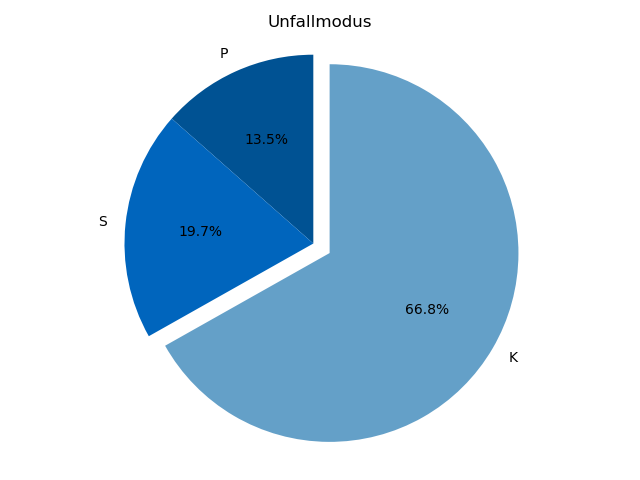
\includegraphics[width=8.1cm,height=6cm]{figures/Unfallmodus}
		\caption[Häufigkeit des Unfallmoduses]{Häufigkeit von Unfällen mit Personenschaden, Unfällen mit schwerwiegendem Sachschaden und Kleinunfällen}\label{fig:Unfallmodus}
	\end{figure}
\end{savenotes}

\subsection{Vorstellung der Teststrecke}\label{subsechtion:Vorstellung der Teststrecke}
Um einen Überblick über die Teststrecke zu bekommen wurde diese zunächst mit dem Fokus auf Eigenschaften, die für die Datenauswertung relevant sein könnten, analysiert. Die gewonnenen Ergebnisse sind in~\autoref{tab:teststecke} stichpunkthaft dargestellt. 

\begin{table}[htpb]
	\scriptsize
	\caption[Analyse der Teststrecke im Münchner Norden.]{Analyse der Teststrecke im Münchner Norden.}\label{tab:teststecke}
	\centering
	\begin{tabular}{l p{3cm} p{3cm} p{3cm}}
		\toprule
		Eigenschaften & Ungererstraße & Leopoldstraße & Schenkendorfstraße \\
		\midrule
		Länge & 1,3 km & 1,5 km & 1,2 km \\
		Kreuzungen mit LSA & 3 & 2 & 2 \\
		Einmündungen mit LSA & 1 & 5 & - \\
		Einmündungen ohne LSA & 12 & 5 & 2 \\
		Abfahrten/Auffahrten & - & - & 7 \\
		Zulässige Geschwindigkeit & 50 km/h & 50 km/h & 60 km/h \\%evtl. nochmals überprüfen.
		ÖPNV Haltestellen & 2 & 3 & - \\
		Fahrspuren je Richtungsfahrbahn & 2 & 2 teilw. 3 & 2 teilw. 4 \\
		Fahrbahntrennung & durchgängiger Grünstreifen & Tram/Grünstreifen & Grünstreifen/bauliche Trennung\\
		Parkplätze im Seitenraum & Längsparkplätze & Längsparkplätze & - \\
		weitere Parkplätze & Parkplatz Münchner Freiheit & Parkhaus Schwabinger Tor & - \\
		Häufig besuchte Punkte & 2 Tankstellen & 2 Tankstellen & Tankstelle\\
		& Ungererbad & 4 Hotels & \\
		& Spielplatz & Discounter & \\
		\bottomrule
	\end{tabular}
\end{table}

Bei den Untersuchungen wurden nur die Abschnitte der drei Straßen betrachtet, die im Testgebiet liegen. Abbildung \ref{fig:Knoten_Testgebiet} stellt die Teststrecke und alle Knotenpunkte, unterteilt nach Kreuzungen mit LSA und Einmündungen mit/ohne LSA, dar. Kreuzungen ohne LSA treten auf der Strecke nicht auf und werden deshalb nicht berücksichtigt. Die Knotenpunkte, welche zwei Straßen der Teststrecke verknüpfen, werden in~\autoref{tab:teststecke} doppelt gezählt. Unter Abfahrten/Auffahrten sind planfreie Knoten im Gebiet zu verstehen. Ein Beispiel stellt die Auffahrt auf die A9 Richtung Berlin von der Schenkendorfstraße aus dar. Als Fahrspuren wurden die Spuren gezählt, die über einen längeren Bereich durchgehend vorhanden sind. Im Bereich von Knotenpunkten können diese aufgeweitet werden. Teilweise ändert sich die Zahl der Spuren auch mit dem Straßenverlauf. Betrachtet man beispielsweise den südlichen Teil der Leopoldstraße, sind zwei Fahrspuren je Richtungsfahrbahn vorhanden und in der Mitte der Straße befindet sich ein Rasengleis für die Tram. Die Tram wird allerdings nur bis zum Schwabinger Tor auf der Leopoldstraße geführt danach biegt sie ab. Hier ändert sich die Anzahl der Fahrspuren von zwei auf drei je Richtungsfahrbahn. Häufig werden auch Unfälle aufgenommen die sich nicht direkt auf einer der drei Straßen ereigneten, sondern z.B. im Bereich einer Tankstelle, die von der Straße aus angefahren werden kann oder auf einem Parkplatz. Deshalb wurden auch solche Punkte bei der Analyse des Gebiets berücksichtigt.

\begin{savenotes}
	\begin{figure}[H]
		\centering
		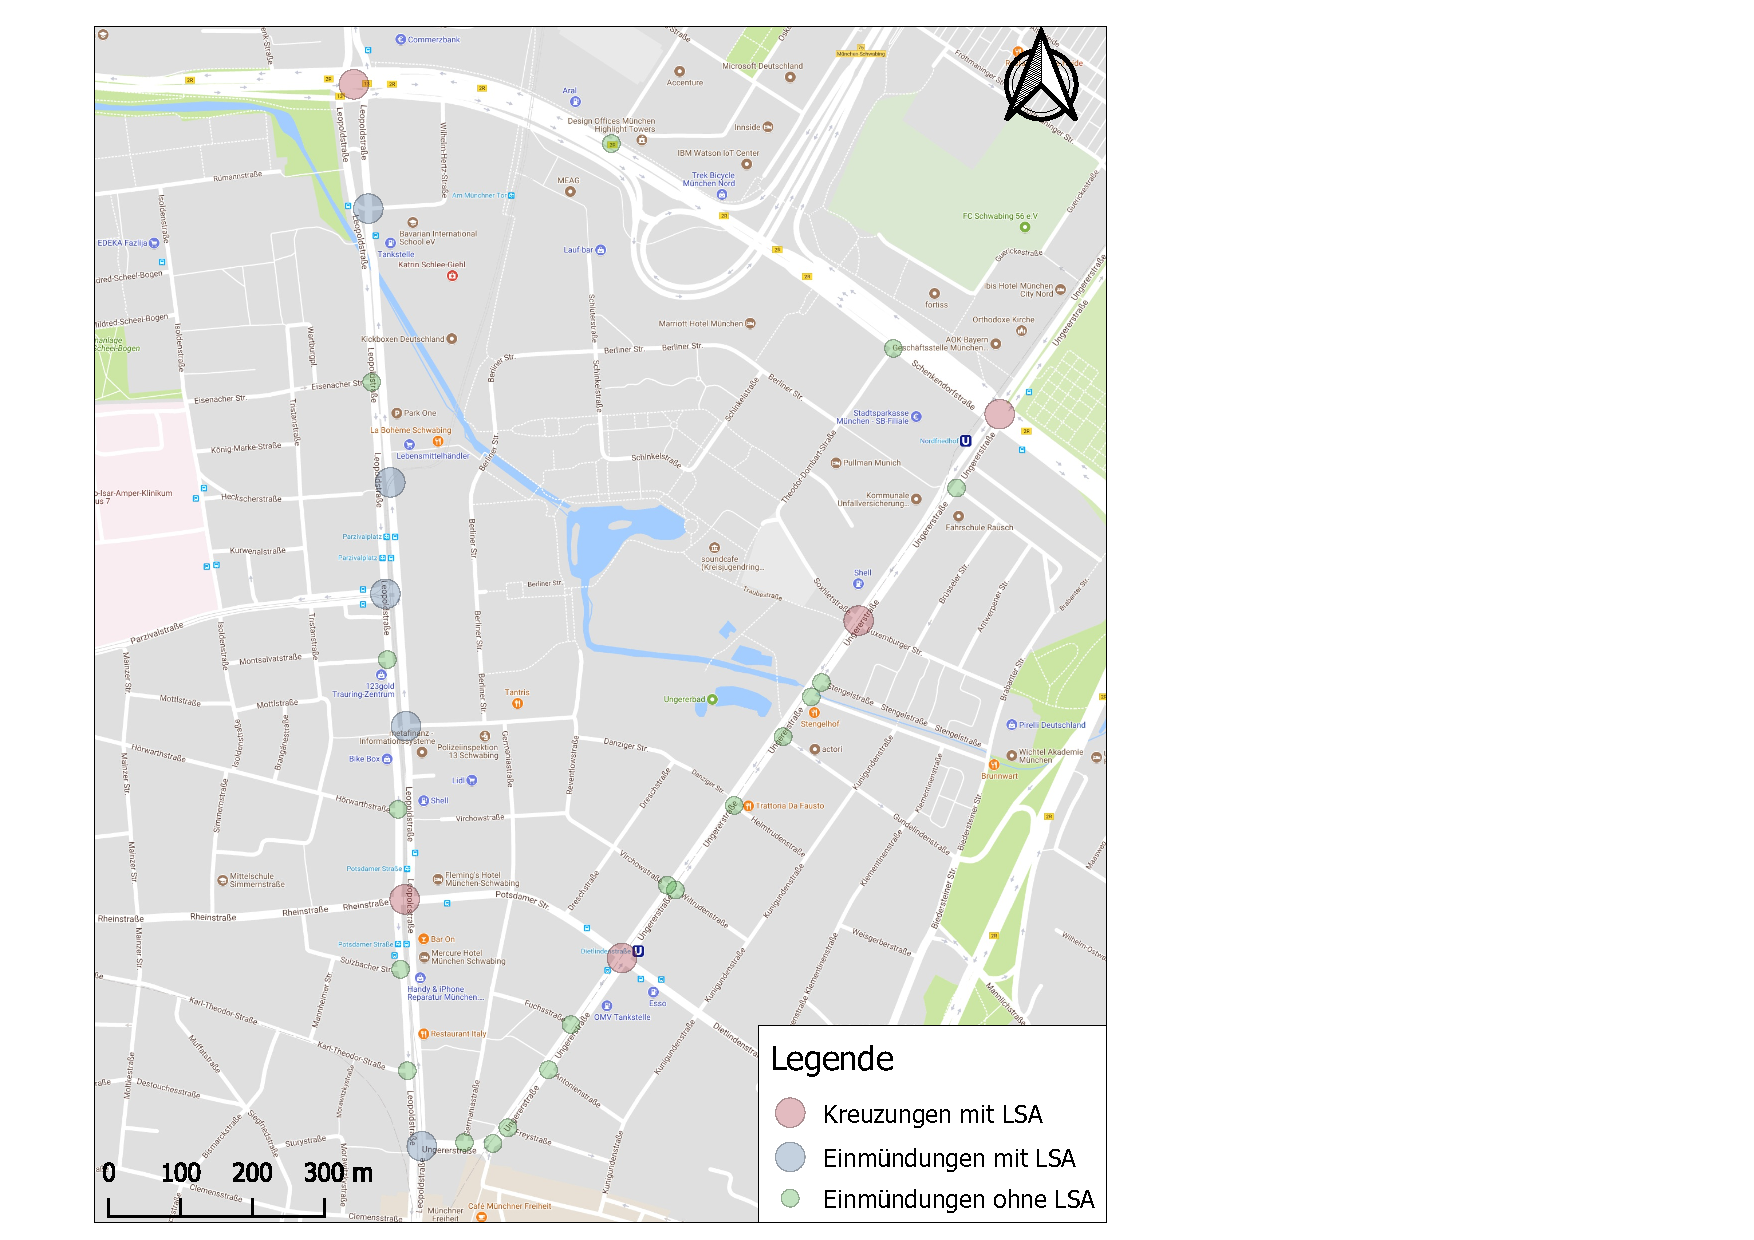
\includegraphics[width=24cm,height=19cm]{figures/Markante_Punkte}
		\caption[Darstellung der Teststrecke, markiert sind die Knotenpunkte, die bei der Analyse berücksichtigt wurden]{Darstellung der Teststrecke, markiert sind die Knotenpunkte, die bei der Analyse berücksichtigt wurden.}\label{fig:Knoten_Testgebiet}
	\end{figure}
\end{savenotes}

%Karte evtl in den Anhang nehmen?

Bei den Kreuzungen und Einmündungen mit LSA soll zusätzlich noch berücksichtigt werden, ob Abbiegestreifen vorhanden sind und ob diese, falls vorhanden, eine eigene Signalisierung für Links- bzw. Rechtsabbieger besitzen. Im Folgenden werden deshalb diese Knotenpunkte noch detaillierter betrachtet. Die Knotenpunktarme der Knoten im Testgebiet sind annähernd rechtwinklig zueinander und werden deshalb in Abbildungen hier immer rechtwinklig zueinander dargestellt.

\subsubsection{Kreuzungen mit LAS}
Es gibt fünf lichtsignalisierte Kreuzungen im Testgebiet. Zwei davon besitzen keine getrennten Abbiegestreifen und werden in diesem Kapitel nicht näher erläutert. Der Knotenpunkt Rheinstraße-Leopoldstraße besitzt an allen Zufahrten einen Abbiegestreifen, hierbei handelt es sich wie in Abbildung \ref{fig:Rhein_Leo} zu erkennen ist um drei Linksabbiegestreifen und einen Rechtsabbiegestreifen. Es gibt jedoch keine eigene Signalisierung für einen der Abbiegestreifen. 

\begin{savenotes}
	\begin{figure}[H]
		\centering
		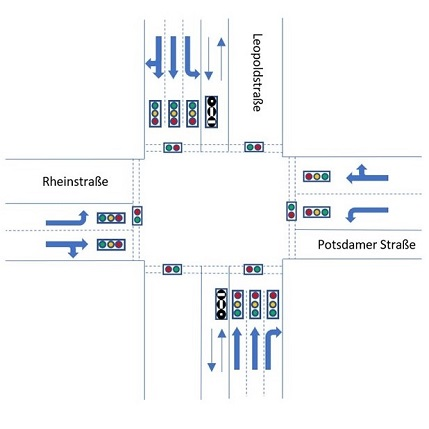
\includegraphics[width=6cm,height=6cm]{figures/Rhein_Leo}
		\caption[Kreuzung Rheinstraße-Leopoldstraße]{Kreuzung Rheinstraße-Leopoldstraße \parencite[S.28]{Kutsch.05.04.2018}.}\label{fig:Rhein_Leo}
	\end{figure}
\end{savenotes}

Die Knotenpunkte Schenkendorfstraße-Ungererstraße und Schenkendorfstraße-Leopoldstraße besitzen dagegen nicht nur mehrere Abbiegestreifen wie in Abbildung \ref{fig:eigene_Signalisierung}
gut zu erkennen ist, sondern teilweise auch eigene Signalphasen für die Abbiegespuren. Diese werden durch Pfeilsymbole an den Ampeln dargestellt. Ein Beispiel für Rechtsabbieger zeigt sich an der Kreuzung Schenkendorfstraße-Leopoldstraße. Wird die Leopoldstraße in Richtung Norden befahren ist beim Rechtsabbiegen auf die Schenkendorfstraße eine eigene Signalisierung vorhanden. Eine eigene Signalisierung für Linksabbieger existiert dagegen an der Kreuzung Schenkendorfstraße-Ungererstraße, wenn man die Ungererstraße in Richtung Norden befährt und links auf die Schenkendorfstraße abbiegt.

\begin{savenotes}
	\begin{figure}[H]
		\centering
		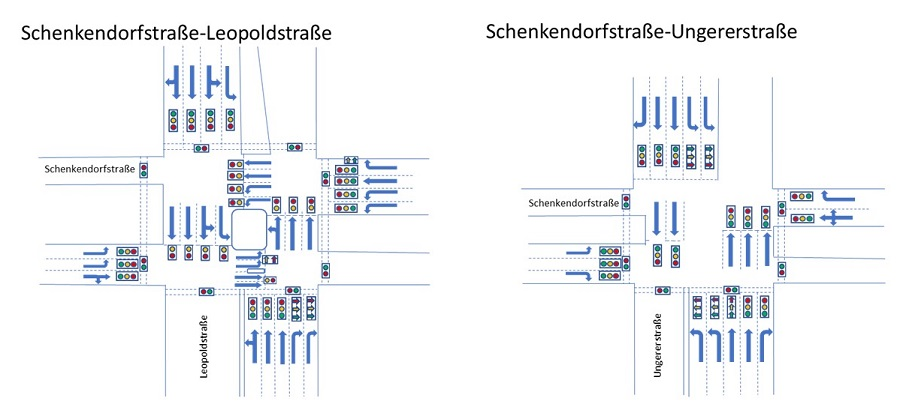
\includegraphics[width=12cm,height=6cm]{figures/Kreuzungen_eigene_Abbiegephase}
		\caption[Kreuzungen mit eigener Signalisierung für Links- bzw. Rechtsabbieger]{Kreuzung mt eigener Signalisierung für Links- bzw. Rechtsabbieger \parencite[S.30-31]{Kutsch.05.04.2018}.}\label{fig:eigene_Signalisierung}
	\end{figure}
\end{savenotes}

\subsubsection{Einmündungen mit LSA}
Innerhalb des betrachteten Gebiets gibt es fünf lichtsignalgeregelte Einmündungen. Eine davon ist die Kreuzung mit der Tram am Schwabinger Tor. Der Kfz-Verkehr kann hier nicht die Richtung wechseln, er folgt weiterhin der Leopoldstraße. Eine weitere besitzt keinen Abbiegestreifen und wird deshalb hier nicht weiter betrachtet. An der Einmündung Leopoldstraße-Ungererstraße gibt es in jedem Knotenpunktarm einen Abbiegestreifen, davon zwei für Linksabbieger und einer für Rechtsabbieger. Diese werden in Abbildung \ref{fig:Einmüngung_Abbiegestreifen} dargestellt.

\begin{savenotes}
	\begin{figure}[H]
		\centering
		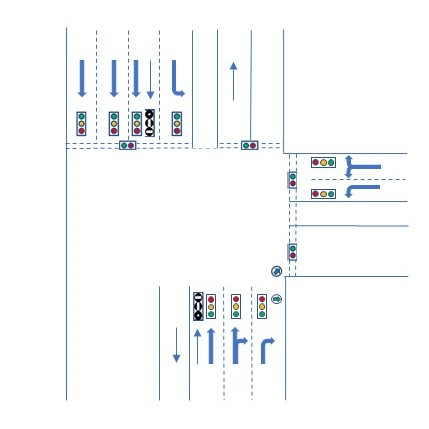
\includegraphics[width=6cm,height=6cm]{figures/Einmuendung_Abbiegestreifen}
		\caption[Einmündung Leopoldstraaße-Ungererstraße]{Einmündung Leopoldstraße-Ungererstraße}\label{fig:Einmüngung_Abbiegestreifen}
	\end{figure}
\end{savenotes}

Einmündungen mit einer eigenen Signalphase für Abbieger stellen die Einmündungen Johann-Fichte-Straße-Leopoldstraße und Parzivalstraße-Leopoldstraße in Abbildung \ref{fig:Einmüngungen_eigene_Phase} dar. Die Einmündung Johann-Fichte-Straße-Leopoldstraße hat einen Rechtsabbiegestreifen ohne eigene Signalisierung und einen Linksabbiegestreifen mit eigener Signalisierung. An der Parzivalstraße gibt es ebenfalls einen Linksabbiegestreifen mit eigener Signalisierung.  

\begin{savenotes}
	\begin{figure}[H]
		\centering
		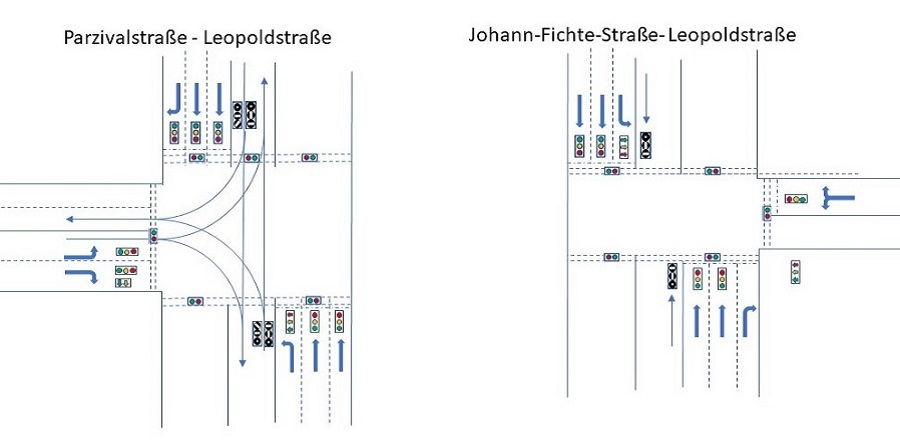
\includegraphics[width=12cm,height=6cm]{figures/Einmuendungen_eigene_Phase}
		\caption[Einmündungen mit eigener Signaphase für Abbieger]{Einmündungen mit eigener Signalphase für Abbieger}\label{fig:Einmüngungen_eigene_Phase}
	\end{figure}
\end{savenotes}

Bis jetzt wurden nur die Knotenpunktbereiche in Nähe der Haltelinien berücksichtigt. Im Bereich der Knotenpunktzufahrt kommt es allerdings ebenfalls häufig zu Konflikten, da hier vermehrt Spurwechsel und Bremsmanöver auftreten. \Textcite[S.19]{Erke.1978} unterteilt die Knotenzufahrt deshalb in drei Segmente, die dann in den Knoteninnenbereich übergehen. Segment 1 beginnt 100 bis 250 m vor dem Knoten mit dem Vorwegweiser und endet mit dem Beginn der Spuraufweitung. Segment 2 erstreckt sich vom Beginn der Spuraufweitung bis zu dem Punkt, an dem alle Spuren voll ausgebildet sind. Segment 3 schließt sich an und reicht bis zur Haltelinie. %Evtl. auch noch bildlich darstellen.


\subsection{Vorstellung der vorhandenen Daten}
Die vorhandenen Unfalldaten für das Testgebiet über die Jahre 2012 bis 2016 beinhalten allgemeine Informationen zu Datum, Uhrzeit und Position des Unfalls. Die Position wird anhand von Geo.-Koordinaten genau angegeben zusätzlich wird noch der Straßennamen und die Hausnummer, bzw. falls es sich um einen Knotenpunkt handelt die Namen beider Straßen, genannt. Die Fahrtrichtung der Fahrzeuge wird, auf die Hausnummern bezogen, mit absteigend oder aufsteigend angegeben.

Um genauere Informationen über die Eigenschaften der Unfallstelle zu bekommen können Charakteristiken und Besonderheiten angegeben werden. Diese Möglichkeit wurde bei den vorhandenen Daten jedoch eher selten genutzt. Ebenso dienen Angaben zu den Lichtverhältnissen, zum Straßenzustand und Geschwindigkeitsbeschränkungen dazu mehr Informationen über Unfallmerkmale zu erhalten.

Um Unfälle besser klassifizieren zu können wird ihnen ein Unfallmodus zugeordnet. Es wird hierbei zwischen drei Unfallmodi unterschieden: Personenschaden, Sachschaden und Kleinunfall. Die Definitionen dazu können Kapitel \ref{subsection:Unfallfolgen} entnommen werden. Neben dem Unfallmodus Personenschaden wird noch angegeben, wie viele Personen sich bei einem Unfall leicht oder schwerverletzt haben bzw. wie viele getötet wurden. Ebenso wird die Höhe des gesamten Sachschadens angegeben.

Weitere Informationen erhält man durch die Angabe des Unfalltyps, der Unfallart und der Unfallursache. Diese wurden in Kapitel \ref{subsection:Begriffe der Unfallaufnahme} definiert. Zusätzlich wird vermerkt, wie viele Personen an einem Unfall beteiligt waren, ob sie unter Drogen- oder Alkoholeinfluss standen und ob es zu einer Unfallflucht kam. 

Bei den Beteiligten wird angegeben in Welcher Art sie am Unfall beteiligt waren z.B. Hauptverursacher, welche Verletzungen sie erlitten haben und welche persönliche Unfallursache vorliegt. Dies ist notwendig, da nicht nur beim Hauptverursacher ein fehlerhaftes Verhalten vorliegen kann.

Die Daten wurden vom Polizeipräsidium München in einer Excel-Datei zur Verfügung gestellt und dienen als Grundlage der Datenanalyse. Selten wurden zu allen oben genannten Positionen angaben gemacht, weshalb die Datei viele Lücken aufweist. Besonders bei Kleinunfällen sind oft nur Angaben zu Datum, Uhrzeit, Position und Unfallursache gegeben. Trotzdem soll versucht werden, so viele Punkte wie möglich bei der Datenanalyse zu berücksichtigen um Fahrsituationen die zu Unfällen führen möglichst genau festzustellen. Eigenschaften die für den späteren Vergleich mit automatisierten Fahrzeugen in \ref{chapter:automatisiertes Fahren} nicht relevant sind wurden zum Teil vernachlässigt. Es wird im Verlauf der Arbeit nicht weiter darauf eingegangen, ob Fahrer unter Drogen- oder Alkoholeinfluss standen und ob es bei dem Unfall zu einer Unfallflucht kam.

\section{Allgemeine Auswertung der Daten}
Um einen Überblick über das Unfallgeschehen innerhalb des Testgebiets zu erhalten eignet es sich zunächst nur die Unfälle, bei denen es zu einem Personen- oder Sachschaden kam zu betrachten. Für Unfälle die als Kleinunfälle aufgenommen wurden liegen wesentlich weniger Informationen vor.

Um eine erste Kategorisierung vorzunehmen eignet sich der Unfalltyp. Dieser gibt Auskunft über die Konfliktsituation. Für die Arbeit von \Textcite[S.16-33]{Bruhn.2018} lagen die Daten des Testgebiets ebenfalls vor. Er hat Karten erstellt, in denen die Unfälle der verschiedenen Unfalltypen auf der kompletten Länge der drei Straße im Testgebiet abgebildet werden. Neben der Lage wurden auch die schwere der Verletzungen und die Hauptverursacher der Unfälle analysiert. In Abbildung \ref{fig:Unfalltyp} wird deshalb nur ein Überblick über die  Anzahl der Unfälle mit zugehörigem Unfalltyp und Unfallmodus innerhalb des betrachteten Zeitraums gegeben. Da hier nur der Bereich der Straßen innerhalb des Testgebiets betrachtet wurde weichen die Ergebnisse zum Teil voneinander ab. 

Am Zweithäufigsten wurde nach dem Unfalltyp 7 \enquote{Sonstiger Unfall} der Typ 6 \enquote{Unfall im Längsverkehr} Bei 26\% der Unfälle angegeben. Hierbei kam es bei 45\% der Unfällen zu einem Personenschaden. Am dritt häufigsten ereigneten sich Unfälle mit dem Unfalltyp 2 \enquote{Abbiege-Unfall}, hierbei kam es in 60\% zu Unfällen mit Personenschaden. 13\% der Unfälle wiesen den Unfalltyp 3 \enquote7Einbiegen/Kreuzen-Unfall auf. Bei diesem Typ handelt es sich an der Einmündung Schenkendorfstraße/Lyonel-Feininger-Straße laut \Textcite[S.23]{Bruhn.2018} um eine kritische Stelle. Unfälle des Typs 4 \enquote{Überschreitunfällle} komme zwar selten für führten aber immer zu einem Personenschaden und ereigneten sich überwiegend in der Leopoldstraße. Hierbei sind vor allem die Bereiche, in denen sich die Tramhaltestellen in der Mitte der Fahrbahn befinden auffällig. Alle Unfälle mit Todesfolge ereigneten sich bei diesem Unfalltyp \parencite[S.26-27]{Bruhn.2018}. Bei dem Typ 5 \enquote{Unfall des ruhenden Verkehrs} kam es dagegen lediglich in 13\% der Unfälle zu einem Personenschaden.

\begin{savenotes}
	\begin{figure}[H]
		\centering
		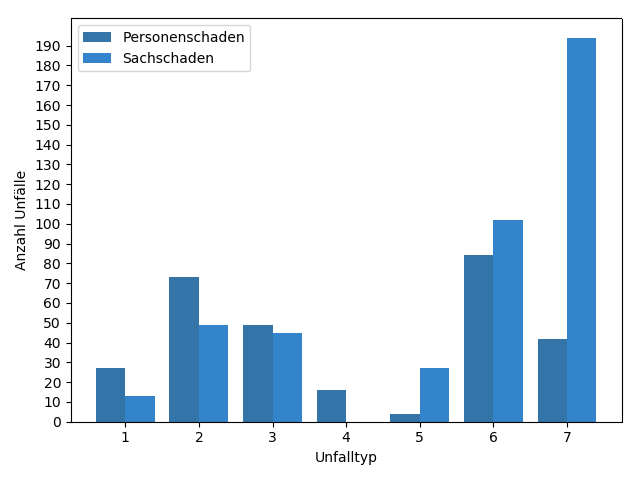
\includegraphics[width=8cm,height=6cm]{figures/Unfalltyp}
		\caption[Unfalltyp der Unfälle, die in den Jahren 2012 bis 2016 im Testgebiet aufgenommen wurden]{Unfalltyp der Unfälle, die in den Jahren 2012 bis 2016 im Testgebiet aufgenommen wurden}\label{fig:Unfalltyp}
	\end{figure}
\end{savenotes}

Um einen Einblick über die Bewegungsrichtung der Fahrzeuge während dem Unfall zu bekommen kann die Unfallart herangezogen werden. Unfällen bei denen ein Personen- oder Sachschaden entstand wurde auch eine Unfallart zugeordnet. Innerhalb des Testgebiets kam es am Häufigsten zu Unfällen bei denen die Unfallart 1 \enquote{Zusammenstoß mit Fahrzeug, das anfährt, anhält oder im ruh. Verkehr steht} angegeben wurde. Bei 26\% der aufgenommenen Unfälle wurde die Unfallart 1 angegeben, bei 22\% die Unfallart 5 \enquote{Zusammenstoß mit Fahrzeug, das einbiegt oder kreuzt}. Währen es bei Unfälle mit der Unfallart 1 Größtenteils nur zu einem Sachschaden kam, hatten mehr als die Hälfte mit der Unfallart einen Personenschaden zur Folge. Am dritthäufigsten ereigneten sich Unfälle mit der Unfallart 3 \enquote{Zusammenstoß mit Fahrzeug, das seitlich oder in gleicher Richtung fährt}. Hierbei kam es in 72\% lediglich zu einem Sachschaden. Die Unfallart 6 \enquote{Zusammenstoß zwischen Fahrzeug und Fußgänger} wurde zwar nur bei 4\% der Unfälle angegeben, es ereignete sich jedoch immer ein Personenschaden. Abbildung \ref{fig:Unfallart} gibt einen Überblick über die Unfallarten und die Unfallschwere, die den Unfällen im Testgebiet zugeordnet wurden.

\begin{savenotes}
	\begin{figure}[H]
		\centering
		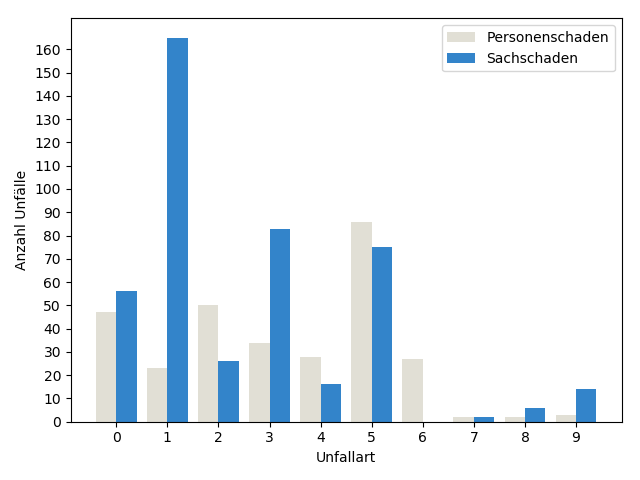
\includegraphics[width=8cm,height=6cm]{figures/Unfallart}
		\caption[Unfallart der Unfälle, die in den Jahren 2012 bis 2016 im Testgebiet aufgenommen wurden]{Unfallart der Unfälle, die in den Jahren 2012 bis 2016 im Testgebiet aufgenommen wurden}\label{fig:Unfallart}
	\end{figure}
\end{savenotes}

Die Beteiligungsart gibt Auskunft darüber, ob ein Unfallbeteiligter Hauptverursacher (BArt01) oder Geschädigter ist (BArt02/BArt03). Innerhalb des Testgebiets wurden nur Unfälle mit bis zu drei Unfallbeteiligten aufgenommen. Die Beteiligungsart wurde nur bei Unfällen bei denen Personen- oder Sachschaden entstand aufgenommen. In 63\% handelte es sich bei den Hauptverursachern um Pkw-Fahrer. Am Zweithäufigsten wurden Unfälle durch unbekannte Fahrzeuge (13\%) ausgelöst, unbekannt wird meisten bei Unfällen mit Fahrerflucht angegeben. An dritter Stelle stehen Lkw-Fahrer mit 10\% als Hauptverursacher. Bei den Unfallgegnern machten ebenfalls die Pkw-Fahrer mit 71\% der größten Anteil aus. An Zweiter Stelle stehen Fahrradfahrer mit 16\%. In Abbildung \ref{fig:Beteiligungsart} werden die Unfälle im Testgebiet nach Beteiligungsart und Art der Verkehrsbeteiligung dargestellt. 

\begin{savenotes}
	\begin{figure}[H]
		\centering
		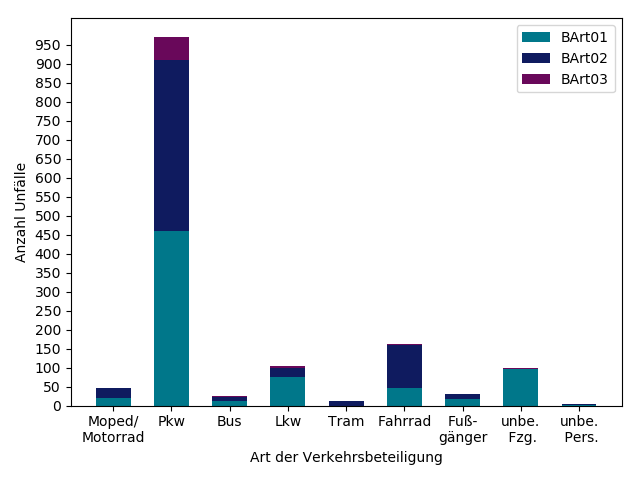
\includegraphics[width=8cm,height=6cm]{figures/BArt}
		\caption[Beteiligungsart der Verkehrsteilnehmer, die bei Unfällen in den Jahren 2012 bis 2016 im Testgebiet angegeben wurden]{Beteiligungsart der Verkehrsteilnehmer, die bei Unfällen in den Jahren 2012 bis 2016 im Testgebiet angegeben wurden}\label{fig:Beteiligungsart}
	\end{figure}
\end{savenotes}

\section{Überprüfung der Hypothesen}\label{sechtion:Überprüfung der Thesen}
In diesem Kapitel werde die in Kapitel \ref{chapter:Methodik} aufgestellten Hypothesen auf ihre Gültigkeit hin überprüft. Da zu vermuten ist, dass die Genauigkeit der Unfallaufnahme mit der Schwere der Unfallfolgen ansteigt und somit die Daten von Personenschadensunfällen verlässlicher sind \parencite[S.11]{StatistischesBundesamt.2018b}. Wird bei der statistischen Auswertung der vorhandenen Unfalldaten der Unfallmodus miteinbezogen. Dieser gibt an, ob es sich um Unfälle mit Personen- bzw. Sachschaden oder um Kleinunfälle handelt. Zusätzlich wird in den meisten Fällen nach bestimmten Unfallursachen differenziert, um den Unfallhergang möglichst genau abzubilden. %Kann man das so als Einleitung stehen lassen?

\subsection{Abbiegeunfälle}
Der Unfalltyp Abbiegeunfälle wurde bei insgesamt 17\% der Unfälle im Untersuchungsgebiet mit Personen oder Sachschaden angegeben. Dabei kam es in 60\% zu Unfällen mit Personenschaden, wie in Abbildung \ref{fig:Unfallart} zu erkennen ist. Der Unfalltyp gibt jedoch keine Auskunft, ob es sich um einen Unfall beim Rechtsabbiegen oder Linksabbiegen handelt. Hierfür werden zusätzlich die Unfallursachen \enquote{Fehler beim Abbiegen nach rechts} (34) und \enquote{Fehler beim Abbiegen nach links} (35) betrachtet. Abbildung \ref{fig:Abbiegen_rechts_links} stellt das Verhältnis der Unfälle, bei denen eine der beiden Ursachen angegeben wurde, dar. Innerhalb des betrachteten Zeitraums ereigneten sich 57,7\% der Unfälle beim Abbiegen nach links und bilden somit die Mehrheit der Abbiegeunfälle.

\begin{savenotes}
	\begin{figure}[H]
		\centering
		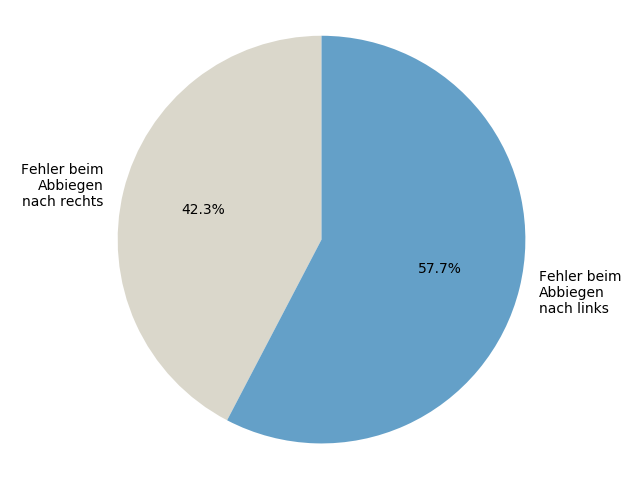
\includegraphics[width=8cm,height=6cm]{figures/These_1}
		\caption[Unfälle bei denen Abbiegefehler nach recht bzw. links in den Jahren 2012 bis 2016 im Testgebiet aufgenommen wurden]{Unfälle bei denen Abbiegefehler nach recht bzw. links in den Jahren 2012 bis 2016 im Testgebiet aufgenommen wurden}\label{fig:Abbiegen_rechts_links}
	\end{figure}
\end{savenotes}

Hierbei wurden alle Unfälle, unabhängig des Unfalltyps, berücksichtigt, denen entweder die Ursache 34 oder 35 zugeordnet wurde. Somit können auch Kleinunfälle, denen kein Unfalltyp zugeordnet wird, berücksichtigt werden. Abbildung \ref{fig:Abbiegen_Md} stellt die Anzahl der Unfälle beim Abbiegen nach links bzw. rechts und den zugehörigen Unfallmodus dar. Vor allem beim Abbiegen nach links kommt es häufig nur zu Kleinunfällen.
Bei der Mehrheit der Unfälle mit Sach- und Personenschaden wurde auch der Unfalltyp 2 angegeben, bei Urs34 in 83\% bei Urs35 in 76\%.

\begin{savenotes}
	\begin{figure}[H]
		\centering
		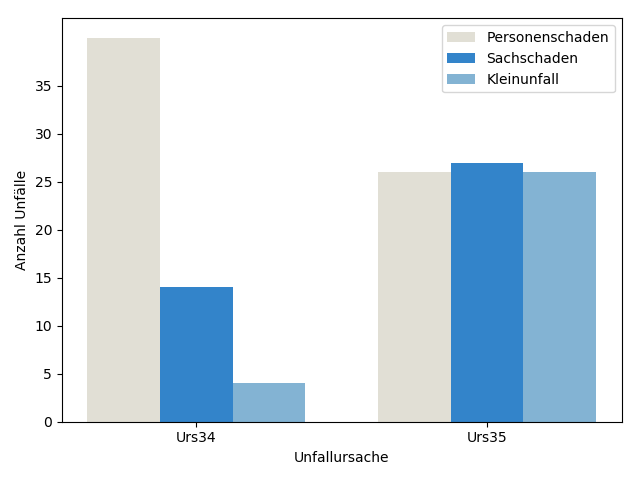
\includegraphics[width=8cm,height=6cm]{figures/Abbiegen_Md}
		\caption[Unfallmodus bei Abbiegeunfällen, die in den Jahren 2012 bis 2016 im Testgebiet aufgenommen wurden]{Unfallmodus bei Abbiegeunfällen, die in den Jahren 2012 bis 2016 im Testgebiet aufgenommen wurden}\label{fig:Abbiegen_Md}
	\end{figure}
\end{savenotes}

Unfälle beim Rechtsabbiegen sind zwar seltener, dafür kommt es zu schwereren Verletzungen. Häufig wird hierbei, wie in Abbildung \ref{fig:Abbiegen_Verletzungen} dargestellt ist, nicht der Hauptverursacher des Unfalls sondern der zweite Unfallbeteiligte verletzt. Dies liegt daran, dass es oft zu Unfällen zw. Pkw-Fahren und Fahrradfahren kommt, vgl. Kapitel \ref{subsection:Abbiegeunfälle mit Radfahrern}. Beim Abbiegen nach links ist die Verletzungsschwere geringer, das sich viele Unfälle zw. zwei Pkws ereignen. \textit{Hypothese 1} gibt an, dass es beim Linksabbiegen mehr Konfliktpunkte gibt und es daher häufiger zu Unfällen kommt als beim Rechtsabbiegen und kann anhand der oben genannten Zahlen bestätigt werden.

\begin{savenotes}
	\begin{figure}[H]
		\centering
		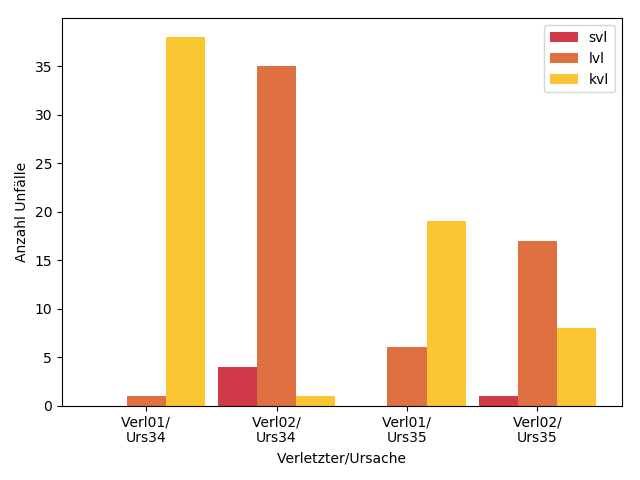
\includegraphics[width=8cm,height=6cm]{figures/Abbiegen_Verletzung}
		\caption[Verletzungsschwere der Unfallbeteiligten bei Abbiegeunfällen, die in den Jahren 2012 bis 2016 im Testgebiet aufgenommen wurden]{Verletzungsschwere bei Abbiegeunfällen, die in den Jahren 2012 bis 2016 im Testgebiet aufgenommen wurden}\label{fig:Abbiegen_Verletzungen}
	\end{figure}
\end{savenotes}

Abbildung \ref{fig:map_Urs35} stellt Unfälle die durch Fehler beim Linksabbiegen entstanden sind dar. Auffällig sind hier vor allem die Knotenpunkte Leopoldstraße/Potsdamer Straße, Schenkendorfstr./Ungererstr. und Leopoldstr./Ungererstraße. Die Knotenpunkte wurden bereits in Kapitel \ref{subsechtion:Vorstellung der Teststrecke} genauer beschrieben. Anhand der Kurzsachverhalte kann man bei fast allen Unfällen auf den genauen Unfallhergang schließen. An der Kreuzung Leopoldstr./Potsdamer Str. ereigneten sich innerhalb der Jahre 2013 bis 2016 insgesamt 16 Unfälle zwischen einem Fahrzeug, dass die Leopoldstr. in südlicher Richtung befuhr und nach links in die Potsdamer Straße abbiegen wollte und einem Fahrzeug, welches die Leopoldstr. geradeaus in nördliche Richtung befuhr. Bei sechs der aufgenommenen Unfälle handelte es sich beim Unfallgegner um Radfahrer. Zusätzlich kam es zu vier Unfällen zwischen Linksabbiegern und einer nachfolgenden Tram. In Abbildung \ref{fig:Rhein_Leo} ist zu erkennen, dass die Kreuzung zwar einen Linksabbiegestreifen besitzt, dieser wird jedoch nicht durch eine eigene Signalphase geregelt. Deshalb kommt es häufig zu Konflikten mit entgegenkommenden Fahrzeugen.

\begin{savenotes}
	\begin{figure}[H]
		\centering
		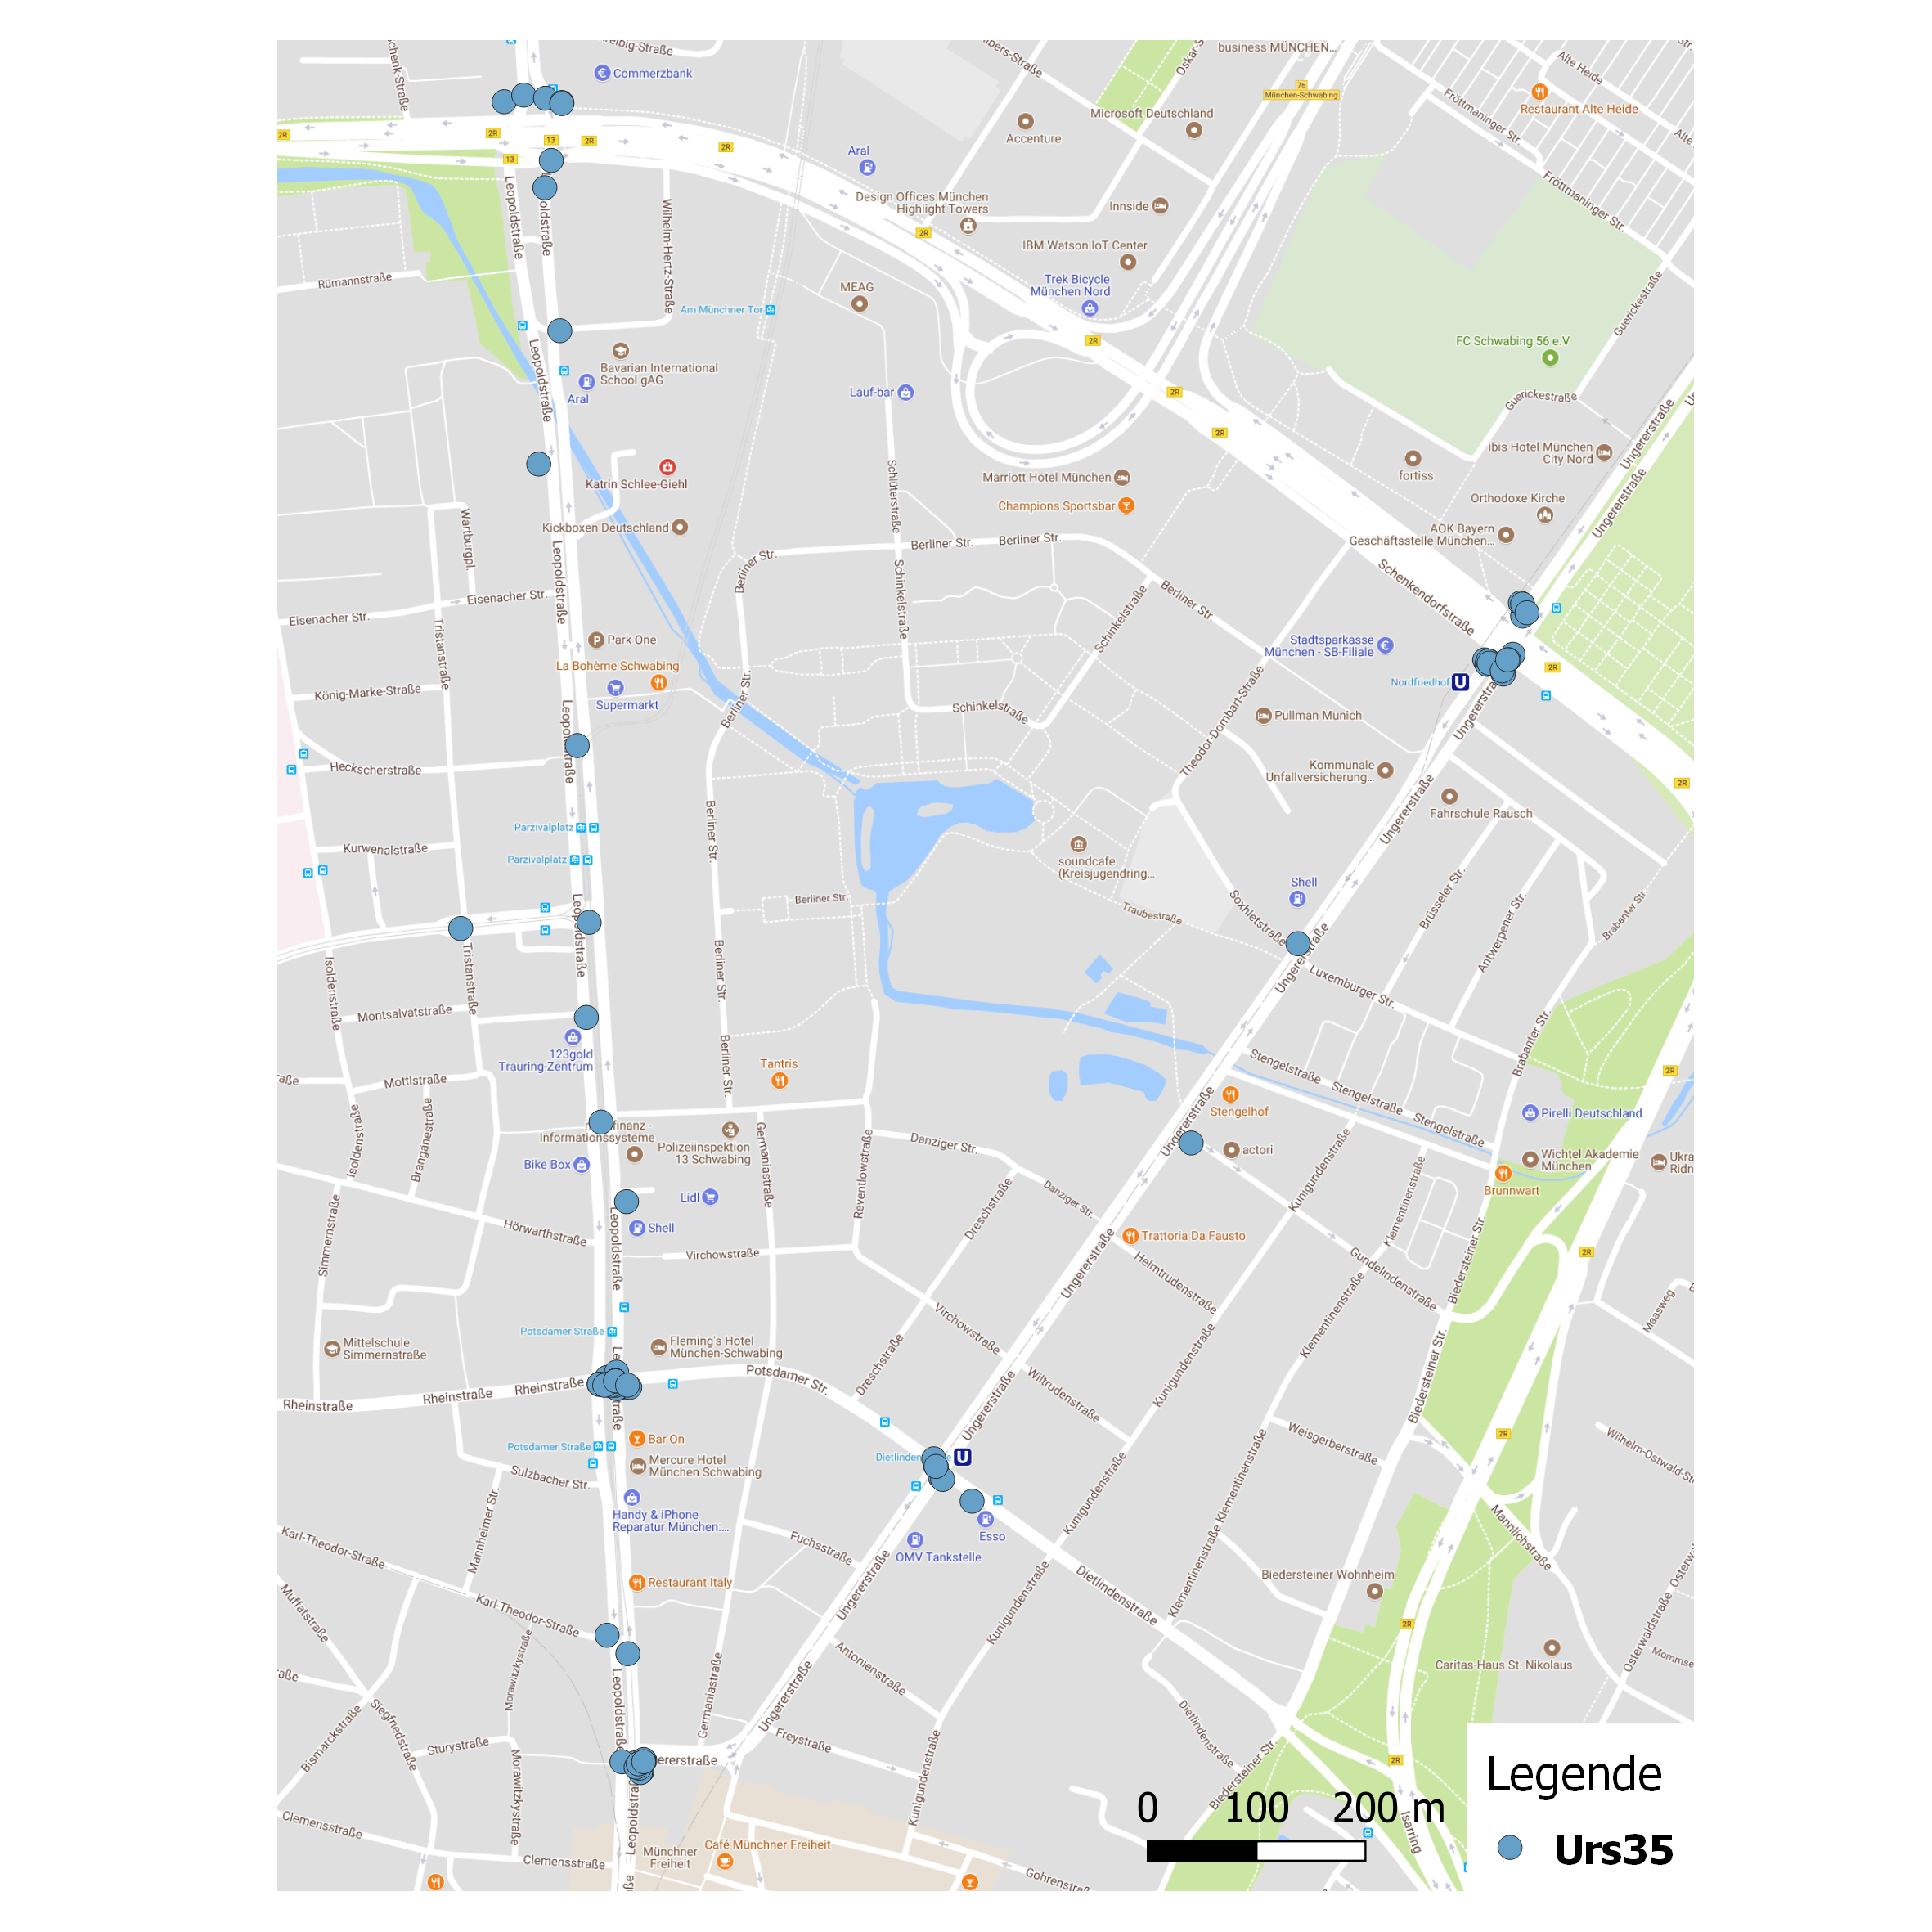
\includegraphics[width=10cm,height=10cm]{figures/map_Urs35}
		\caption[Unfälle durch Fehler beim Linksabbiegen, die in den Jahren 2012 bis 2016 im Testgebiet aufgenommen wurden]{Unfälle durch Fehler beim Linksabbiegen, die in den Jahren 2012 bis 2016 im Testgebiet aufgenommen wurden}\label{fig:map_Urs35}
	\end{figure}
\end{savenotes}

Die Kreuzung Ungererstraße/Schenkendorfstraße besitzt Linksabbiegestreifen mit eigener Signalphase (Abbildung  \ref{fig:eigene_Signalisierung}). Eine Phase ist für die Ungererstr. in südliche Fahrtrichtung und eine für die Ungererstr. in nördliche Fahrtrichtung. Trotzdem sieht es so aus als würden sich an dieser Kreuzung ähnlich viele Unfälle ereignen wie an der zuvor diskutierten. Betrachtet man die Unfälle genauer, handelt es sich vor allem um Unfälle mit Fahrzeugen die in die gleiche Richtung fahren. Die Linksabbieger werden auf zwei Linksabbiegestreifen geführt, wird die Fahrspur beim abbiegen nicht eingehalten kommt es zum Zusammenstoß. Unfälle mit entgegenkommenden Fahrzeugen konnten nur in vier Fällen ausgemacht werden. Diese ereigneten sich durch nicht verkehrsgerechtes Wenden.

Die Einmündung Leopoldstraße/Ungererstraße besitzt keine eigene Signalphase für Linksabbieger (Abbildung \ref{fig:Einmüngung_Abbiegestreifen}). Hier ereigneten sich in den Jahren 2013 bis 2016 fünf Unfälle zwischen Fahrzeugen, welche den Abbiegestreifen auf der Leopoldstraße in südliche Richtung befuhren um nach links in die Ungererstr. abzubiegen und entgegenkommenden Fahrzeugen. An den Einmündungen mit einer eigenen Signalphase für Linksabbieger, die in der Abbildung \ref{fig:Einmüngungen_eigene_Phase} dargestellt werden. Ereignete sich lediglich ein Unfall im Untersuchungszeitraum. Hierbei handelt es sich um einen Auffahrunfall, welcher durch zu starkes Bremsen beim Abbiegevorgang ausgelöst wurde.

\begin{table}[htpb]
	\scriptsize
	\caption[Verkehrsstärken an ausgewählten Linksabbiegestreifen im Testgebiet]{Verkehrsstärken an ausgewählten Linksabbiegestreifen im Testgebiet}\label{tab:Linksabbieger}
	\centering
	\begin{tabular}{l p{3cm} p{3cm} }
		\toprule
		Knotenpunkt & Linksabbiegestreifen & Verkehrsstärke \\
		\midrule
		Leopoldstr./Potsdamer Str. & Leopold in südl. Richtung & 2084 [Kfz/Tag] \\
		Leopoldstr./Parzivalstr. & Leopold in nördl. Richtung & 2027[Kfz/Tag] \\
		Leopoldstr./Ungererstr. & Leopold in südl. Richtung & 2206 [Kfz/Tag] \\
		\bottomrule
	\end{tabular}
\end{table}

Neben den Unfällen wurden an den Knotenpunkten in der Leopoldstraße auch die Verkehrsstärken berücksichtigt. Für die Kreuzung Ungererstraße/Schenkendorfstraße liegen leider keine Werte vor. Es wurden an den Kreuzungen jeweils die Messwerte von Detektoren der Linksabbiegerstreifen betrachtet. Als Referenz wurde Donnerstag der 7.5.2016 bzw. 3.5.2018 gewählt. Hierbei handelt es sich um einen Arbeitstag außerhalb der Schulferien. Der Einfachheit halber wurde zum Vergleich die Tagessumme der Messwerte verwendet. Diese wird in Tabelle \ref{tab:Linksabbieger} dargestellt. Die Verkehrsstärken der Knoten Leopoldstr./Reihnstr. und Leopoldstr./Parzivalstr. weichen nur minimal voneinander ab. Trotzdem ereignen sich an erstgenanntem Knoten wesentlich mehr Unfälle. Die Daten für die Einmündung Untererstr./Leopoldstr. sind aus dem Jahr 2018 und weißen eine etwas höhere Verkehrsstärke auf. Es ist anzunehmen, dass sich die Verkehrsstärke innerhalb zwei Jahren etwas erhöht hat. Die Verkehrsstärke im Jahr 2016 sollte hier also ähnlich gewesen sein, wie an den anderen zwei Knotenpunkten. Trotzdem ereigneten sich an der Einmündung mit der Ungererstraße mehr Unfälle als an der Parzivalstraße. 
 
\begin{savenotes}
	\begin{figure}[H]
		\centering
		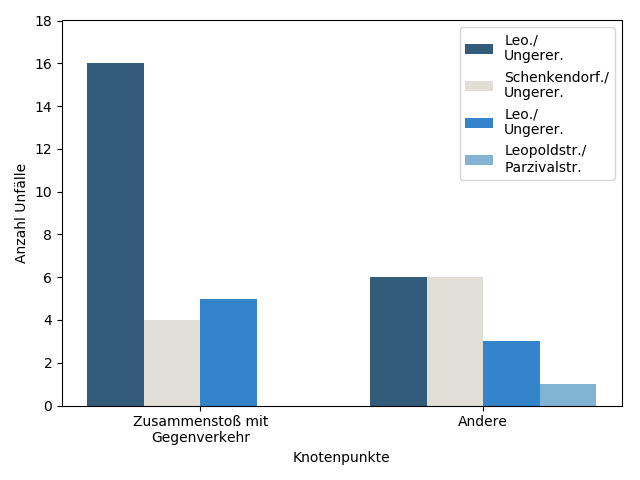
\includegraphics[width=8cm,height=6cm]{figures/Unfaelle_Signalphasen}
		\caption[Linksabbiegeunfälle an Knotenpunkten mit und ohne eigene Signalisierung, die in den Jahren 2013 bis 2016 im Testgebiet aufgenommen wurden]{Linksabbiegeunfälle an Knotenpunkten mit und ohne eigene Signalisierung, die in den Jahren 2013 bis 2016 im Testgebiet aufgenommen wurden}\label{fig:Unfaelle_Signalphasen}
	\end{figure}
\end{savenotes}

\textit{Hypothese 2} gibt an, dass sich die Konfliktpunkte und Unfallzahlen reduzieren, wenn Linksabbieger, an Kreuzungen mit LSA, auf einem eigenen Fahrstreifen mit eigener Signalphase geführt werden. Betrachtet man die Zahlen in Abbildung \ref{fig:Unfaelle_Signalphasen} kommt es in 73\% an Kreuzungen ohne eigene Signalisierung zu Unfällen beim Linksabbiegen. In 70\% handelt es sich dabei um Unfälle mit entgegenkommenden Fahrzeugen. Vor allem dieser Konflikt kann durch eine eigene Phase deutlich reduziert werden. \textit{Hypothese 2} kann daher bestätigt werden.

\subsection{Unfälle während der Hauptverkehrszeiten}
Laut \Textcite[S.80-81]{StatistischesBundesamt.2017} ereigneten sich die meisten Unfälle im Jahr 2016 innerhalb von Ortschaften, bei denen es zu einem Personenschaden kam, von Montag bis Freitag zwischen 7 und 20 Uhr. In den morgen Stunden kommt es zwischen sieben und acht am häufigsten zu Unfällen. Auffällig ist, dass keine deutlichen Spitzen zu den vermuteten Hauptverkehrszeiten (Vormittags/Nachmittags) zu erkennen sind.  Die Zahl der Unfälle steigt nach einem leichten Rückgang am Vormittag schon zur Mittagszeit gegen elf Uhr wieder an. Am Nachmittag ereignen sich die meisten Unfälle zwischen 16 Uhr und 18 Uhr. Auffällig ist auch, dass sich mehr Unfälle am Nachmittag als am Vormittag ereignen. An Wochenenden kommt es seltener zu Unfälle, dafür ist die Anzahl in den Nächten von Freitag auf Samstag und von Samstag auf Sonntag höher als unter der Woche.

Für das Testgebiet stehen zum Teil Messwerte von Detektoren an Knotenpunkten zur Verfügung. \Textcite[S.10-16]{Bruhn.2018} hat anhand dieser Daten ermittelt, wann die Verkehrsmengen auf den einzelnen Straßen am höchsten sind. In der Leopoldstraße ist die Verkehrsmenge grundsätzlich von 8 bis 19 Uhr erhöht. Einzelne Spitzen sind am Vormittag zwischen 8 und 10 Uhr und Abends zw. 18 und 19 Uhr zu erkennen. Diese sind jedoch sehr gering ausgeprägt. Auf der Ungererstraße ist das Verkehrsaufkommen zwischen 7 und 9 Uhr sowie zw. 16 und 19 Uhr erhöht. In den Zeiträumen von 7 bis 9 Uhr und 17 bis 19 Uhr konnte auf der Schenkendorfstraße ein erhöhtes Verkehrsaufkommen festgestellt werden. Bei den Detektordaten werden nicht motorisierte Verkehrsteilnehmer vernachlässigt, da an Rad- bzw. Fußgängerüberwegen keine Detektoren vorhanden sind.

\begin{savenotes}
	\begin{figure}[H]
		\centering
		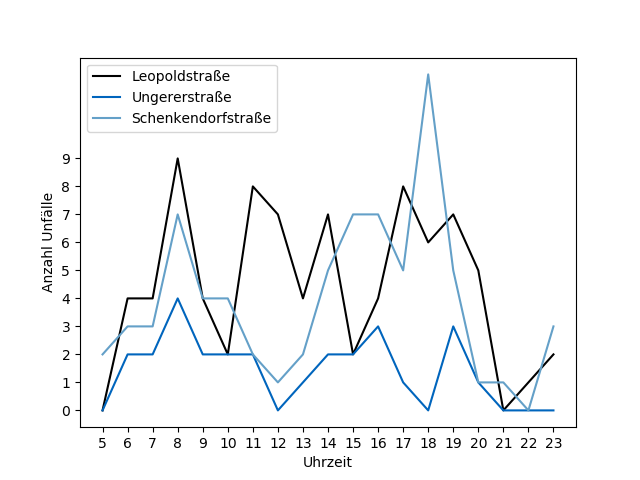
\includegraphics[width=8cm,height=6cm]{figures/Typ6}
		\caption[Zeitliche Verteilung der Unfälle mit Unfalltyp 6 in den Jahren 2012 bis 2016 innerhalb des Testgebiets]{Zeitliche Verteilung der Unfälle mit Unfalltyp 6 in den Jahren 2012 bis 2016 innerhalb des Testgebiets}\label{fig:Unfalltyp6_Uhrzeit}
	\end{figure}
\end{savenotes}

\textit{Hypothese 3} gibt an, dass bei höherem Verkehrsaufkommen, die Anzahl der Verkehrsunfälle im Längsverkehr steigt. Zu Überprüfung der These werden hier nur die Unfälle betrachtet, bei denen der Unfalltyp 6 angegeben wurde. Der Zeitliche Verlauf aller Unfälle im Testgebiet wurde bereits von \Textcite[S.10-16]{Bruhn.2018} analysiert. In Abbildung \ref{fig:Unfalltyp6_Uhrzeit} ist zu erkennen, dass Unfälle im Längsverkehr auf der Leopoldstraße zwischen 8 und 20 Uhr erhöht auftraten. Auf der Ungererstraße ereigneten sich innerhalb des Untersuchungszeitraums insgesamt nur 27 Unfälle mit dem Unfalltyp 6. Daher ist es schwer Zeitpunkte mit erhöhtem Verkehrsaufkommen zu bestimmen. Zwischen 8 und 9 Uhr, 16 und 17 Uhr sowie 19 und 20 Uhr sind leichte Spitzen zu erkennen. Auf der Schenkendorfstraße kam es Vormittags zwischen 8 und 11 Uhr sowie Nachmittags zwischen 14 und 20 Uhr vermehrst zu Unfällen im Längsverkehr. Am meisten Unfälle ereigneten sich zwischen 18 und 19 Uhr. Vergleicht man die Zeiträume in denen sich Unfälle ereigneten mit den Messwerten der Detektoren, stimmen diese nur zum Teil überein. Auf der Leopoldstraße wurde sowohl ein erhöhtes Verkehrsaufkommen als auch erhöhte Unfallzahlen über den gesamten Tag festgestellt werden. Die Unfallzahlen der Ungererstraße sind für einen konkreten Vergleich zu gering und auf der Schenkendorfstraße stimmen die Bereiche fast überein. Die Zeiträume in denen es vermehrt zu Unfällen kommt sind jedoch größer als diejenigen mit erhöhtem Verkehrsaufkommen. Zusammenfassend sind die Daten nicht aussagekräftige genug um \textit{Hypothese 3} vollständig bestätigen zu können.

\begin{savenotes}
	\begin{figure}[H]
		\centering
		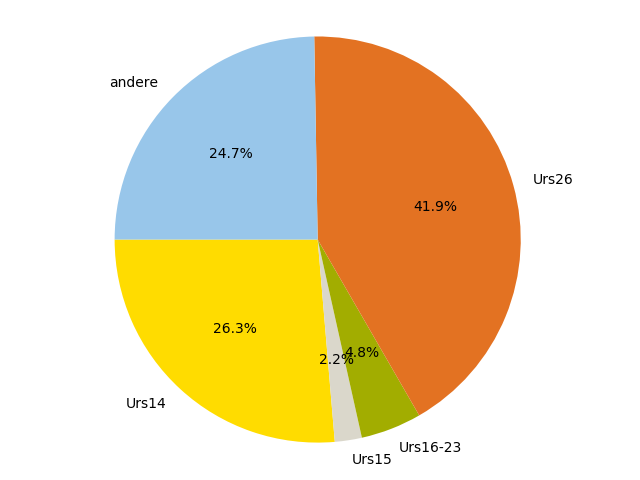
\includegraphics[width=8cm,height=6cm]{figures/Urs_Typ6}
		\caption[Unfallursachen, die Unfällen im Längsverkehr innerhalb des Testgebiets zugeordnet wurden]{Unfallursachen, die Unfällen im Längsverkehr innerhalb des Testgebiets zugeordnet wurden}\label{fig:Unfallursachen_Unfalltyp6}
	\end{figure}
\end{savenotes}

\textit{Hypothese 3} gibt zudem an, dass sich Unfällen im Längsverkehr hauptsächlich durch Konflikte beim Spurwechsel und durch zu geringen Sicherheitsabstand ereignen. Hierfür wurden die Unfallursachen betrachtet, die angegeben werden können, wenn beim Fahrzeugführer Fehler auftraten, die auf den Abstand, Überholen oder das Nebeneinanderfahren zurückzuführen sind. Bei 75\% der Unfälle im Längsverkehr wurde eine dieser Ursachen angegeben. Am häufigsten kam es dabei zu Unfällen, aufgrund von Fehlern beim Fahrstreifenwechsel (Ursache 26). Diese Ursache wurde bei 42\% der Unfälle mit Unfalltyp 6 angegeben. Gefolgt von der Ursache 14 \enquote{ungenügender Sicherheitsabstand}, welche bei 26\% genannt wurde. Fehler beim Überholen wurden lediglich bei 5\% notiert. Bei 2\% der Unfälle wurde die Ursache 15 \enquote{Starkes Bremsen des Vorausfahrenden ohne zwingenden Grund} angegeben. Bei 46 Unfällen (25\%) wurden Ursachen angegeben, die auf auf den ersten Blick nicht auf Unfälle im Längsverkehr hinweisen. Abbildung \ref{fig:Unfallursachen_Unfalltyp6} werden die Unfallursachen, der Unfälle im Längsverkehr angegeben. Die häufige Nennung der Unfallursachen, die auf Fehler beim Spurwechsel oder zu geringen Sicherheitsabstand hinweisen führt dazu, dass \textit{Hypothese 3} in diesem Punkt bestätigt werden kann.

\begin{savenotes}
	\begin{figure}[H]
		\centering
		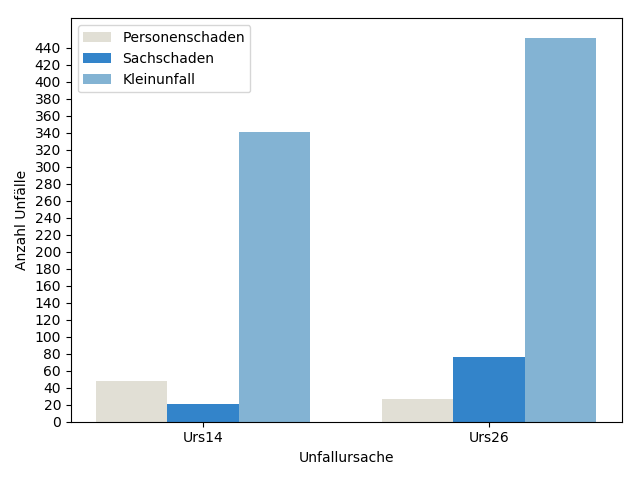
\includegraphics[width=8cm,height=6cm]{figures/Urs14_Urs26_Md}
		\caption[Schwere der Unfälle, bei denen als Unfallursache Ungenügender Sicherheitsabstand bzw. Fehler beim Spurwechsel angegeben wurden]{Schwere der Unfälle, bei denen als Unfallursache Ungenügender Sicherheitsabstand bzw. Fehler beim Spurwechsel angegeben wurden}\label{fig:Unfallursachen_14_26}
	\end{figure}
\end{savenotes}

Betrachtet man nur die Unfallursachen 14 und 26 ohne Unfalltyp können auch Kleinunfälle mit berücksichtigt werden. Diese machen hier, wie in Abbildung \ref{fig:Unfallursachen_14_26} zu erkennen ist, mit \% bei Ursache 26 bzw. \% bei Ursache 14 einen erheblichen Anteil aus. Auffällig ist zudem, dass es zwar seltener zu Unfällen durch zu geringen Sicherheitsabstand kam, diese führten dafür häufiger zu Personenschaden, als die Unfälle beim Spurwechsel.

\subsection{Unfälle durch ruhenden Verkehr}
Unfälle des ruhenden Verkehrs stellen den Unfalltyp 5 in Abbildung \ref{fig:Unfalltyp} dar. Im Untersuchungszeitraum wurden 31 Unfälle von diesem Typ aufgenommen. Bei lediglich 13\% davon kam es zu einem Personenschaden. Ein Unfalltyp wurde nur den Unfällen mit Personen- bzw. Sachschaden zugeordnet. Bei Kleinunfällen kann man nur anhand von angegebenen Unfallursachen darauf schließen, ob es sich um einen Unfall durch ruhenden Verkehr handelt. Betrachtet man zunächst die Unfälle denen ein Unfalltyp zugeordnet wurden ereigneten sich ca. 61\% auf der Leopoldstraße, 29\% auf der Ungererstraße und 10\% auf der Schenkendorfstraße. 

Eine weiter Möglichkeit Parkunfälle zu identifizieren ist die Unfallursache \enquote{Zusammenstoß mit Fahrzeug, das anfährt, anhält, im ruh. Verkehr steht} (1). Die Anzahl der Unfälle bei denen die Unfallart 1 angegeben wurde ist, wie in Abbildung \ref{fig:Unfallart} zu erkennen ist, mit insgesamt 187 Stück wesentlich höher als die Anzahl Unfälle, bei denen der Unfalltyp 5 angegeben wurde. Trotzdem ist das Verhältnis von Personen- zu Sachschaden sehr ähnlich, ebenso die Verteilung der Unfälle auf die drei Straßen des Untersuchungsgebiets. 

Entlang der Leopold- und Ungererstraße sind innerhalb des Testgebiets Längsparkplätze auf beiden Seiten vorhanden. Die erhöhte Anzahl der Unfälle durch ruhenden Verkehr in der Leopoldstraße kann dadurch erklärt werden, dass die Leopoldstraße in einem Mischgebiet liegt. Geschäfte führen zu Kurzparkverkehr. In der Ungererstraße ist überwiegend Wohnnutzung zu erkenne, hier wird der Parkverkehr daher überwiegend durch Anwohnerparken geprägt. Die geringe Anzahl der Unfälle durch ruhenden Verkehr auf der Schenkendorfstraße kann dadurch erklärt werden, dass es keine Parkmöglichkeiten im Seitenraum gibt. \textit{Hypothese 4} gibt an, dass es im urbanen Raum häufig zu Konflikten mit Fahrzeugen im ruhenden Verkehr kommt. Besonders auffällig sind Bereiche mit Längsaufstellung am Fahrbahnrand. Dieser Punkt kann hier zum Teil bestätigt werden. Die Bereiche mit Längsparkplätzen weisen zwar mehr Unfälle durch ruhenden Verkehr auf, jedoch weichen die aufgenommenen Unfallzahlen trotz ähnlicher Parkstruktur stark voneinander ab. Es kommt also nicht nur auf die Anordnung der Parkplätze im Seitenraum an, sondern auch auf die Höhe des Verkehrsaufkommens und der Siedlungsstruktur.

Zusätzlich gibt die \textit{Hypothese 4} an, dass verbotswidriges auf der Straße Halten/Parken eine bedeutende Rolle bei Unfällen im Ruhenden Verkehr spielt, da beim Vorbeifahren kritische Situationen entstehen, die Unfälle auslösen. Als Beispiel wird Parken in Zweiter Reihe genannt. Betrachtet man zunächst die Unfallursachen der Unfälle mit Unfalltyp 5, wurde in 71\% der Fälle \enquote{andere Fehler beim Fahrzeugführer} (49 )angegeben. Bei den Unfällen mit der Unfallart 1 überwiegt ebenso die Ursache 49.
 Da diese Ursache keine Aussagekraft besitzt werden Unfallursachen, die dem ruhenden Verkehr zugeordnet werden direkt betrachtet. Eine davon ist \enquote{unzulässiges Halten oder Parken} (43). Diese wurde jedoch nur zwei mal innerhalb des Untersuchungszeitraums einem Unfall zugeordnet und liefert daher keine ausreichende Auskunft. Etwas häufiger, insgesamt 17 mal, wurde die Ursache \enquote{verkehrswidriges Verhalten beim Ein- oder Aussteigen, Be- und Entladen} angegeben. Hierbei kam es jedoch in 15 Unfällen nur zu Kleinunfällen. Diese Ursache könnte allerdings auf Unfälle mit Lieferverkehr hinweisen die, ähnlich wie in Abbildung \ref{fig:Parken_zweite_Reihe} zu erkennen ist, in der zweiten Reihe parken/halten. Die Aufnahme in Abbildung \ref{fig:Parken_zweite_Reihe} wurde bei einer Ortsbegehung aufgenommen. Keinem der Unfälle bei denen eine der beiden Ursachen angegeben wurde wurde gleichzeitig der Unfalltyp 5 zugeordnet, dafür immer die Unfallart 1. Eine weiter Unfallursache, die auf Unfälle, mit Fahrzeugen welche auf der Straße Halten, hindeutet ist \enquote{Nichtbeachten des nachfolgenden Verkehrs beim Vorbeifahren an haltenden Fahrzeugen} (25). Sie wurde bei vier Unfällen mit Sachschaden, wovon nur einem Unfall gleichzeitig die Unfallart 1 zugeordnet wurde, und fünf Kleinunfällen angegeben. Da die Anzahl der Unfälle, denen die oben genannten Ursachen zugeordnet wurden gering ist, kann \textit{Hypothese 4} hier nicht bestätigt werden. Um herauszufinden, welche Unfälle sich wirklich durch verbotswidriges Halten/Parken ereignet haben müssten genauere Beschreibungen zu den Unfällen vorliegen. % Falls noch Zeit ist, die Kurzbeschreibungen durchzugehen. Diesen Satz ersetzen, ob sich daraus was ergeben hat.

%Ist der Plot wirklich aussagekräftig genug? Bis jetzt auch nicht darauf verwiesen. Wird wahrscheinlich rausgenommen. 
\begin{savenotes}
	\begin{figure}[H]
		\centering
		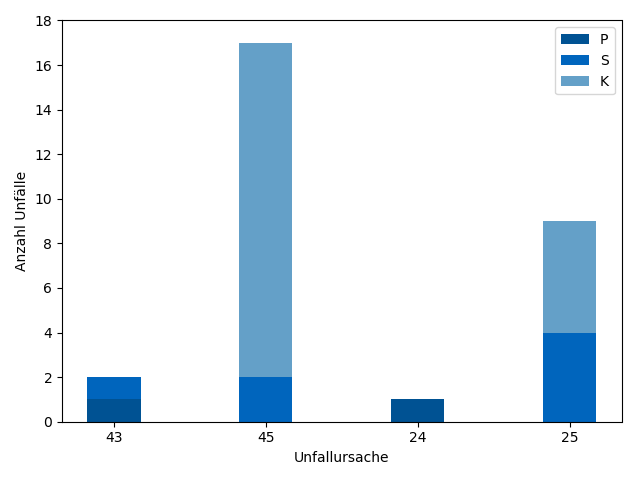
\includegraphics[width=8cm,height=6cm]{figures/Urs_Parken}
		\caption[Unfallursachen die Auskunft über Unfälle im Ruhenden Verkehr geben können, die bei Unfällen in den Jahren 2012 bis 2016 im Testgebiet aufgenommen wurden]{Unfallursachen die Auskunft über Unfälle im Ruhenden Verkehr geben können, die bei Unfällen in den Jahren 2012 bis 2016 im Testgebiet aufgenommen wurden}\label{fig:Unfallursachen_ruhender_Verkehr}
	\end{figure}
\end{savenotes}

\begin{savenotes}
	\begin{figure}[H]
		\centering
		\includegraphics[width=8cm,height=6cm]{figures/zweite_Reihe}
		\caption[Parken in zweiter Reihe auf der Ungererstraße, zu Be- bzw. Entladen]{Parken in zweiter Reihe auf der Ungererstraße, zu Be- bzw. Entladen}\label{fig:Parken_zweite_Reihe}
	\end{figure}
\end{savenotes}

\subsection{Unfälle mit ungeschützten Verkehrsteilnehmern}
Betrachtet man Abbildung \ref{fig:Beteiligungsart} ist zu erkennen, dass der Anteil an Unfällen an denen Fahrradfahrer, Fußgänger oder unbekannte Personen, sogenannte ungeschützte Verkehrsteilnehmer, beteiligt waren gering ist. Die Beteiligungsart wurde nur für Unfälle mit Sach- oder Personenschaden angegeben. Es kann daher anhand der vorliegenden Unfalldaten nicht ausgewertet werden, wie viele ungeschützte Verkehrsteilnehmer an Kleinunfällen beteiligt waren. Unfälle mit Moped/Motorrad Beteiligung sollen hier auch zu den ungeschützten Verkehrsteilnehmern gezählt werden. Insgesamt gab es innerhalb des Untersuchungszeitraums 725 Unfälle bei denen es zu einem Personen oder Sachschaden kam. Die Anzahl der Unfälle stimmt nur mit der Summer der Hauptbeteiligten überein, da auch Alleinunfälle aufgenommen wurden. Betrachtet man zunächst die Hauptunfallverursacher wurden 88\% der Unfälle durch motorisierte Verkehrsteilnehmer (ohne Moped/Motorrad) ausgelöst. Lediglich in 12\% der Fälle waren ungeschützte Verkehrsteilnehmer Hauptverursacher. In 654 Fällen gab es mindesten zwei Unfallbeteiligte, hier betrug der Anteil an motorisierten Fahrzeugen 76,5\%, an ungeschützten Verkehrsteilnehmern 23,5\%. Unfälle mit drei Unfallbeteiligten gab es innerhalb des Untersuchungszeitraums nur 71 Stück. Dabei wurden bei 97\% der Unfälle motorisierte Verkehrsteilnehmer als dritte Beteiligungsart angegeben.

\textit{Hypothese 5} gibt an, dass die Komplexität, und somit die Zahl der Unfälle, einer Fahrsituation erhöht wird, sobald nicht motorisierte Verkehrsteilnehmer daran beteiligt sind. Betrachtet man die Art der Verkehrsbeteiligung im Untersuchungsgebiet kann dies nicht bestätigt werden. Der Anteil an motorisierten Verkehrsteilnehmern sowohl als Hauptverursacher eines Unfalls als auch als weiterer Unfallbeteiligte ist deutlich höher als der der nicht motorisierten Verkehrsteilnehmer, hier als ungeschützt bezeichnet. 

Hierbei muss berücksichtigt werden, dass die Teststrecke mit der Schenkendorfstraße einen Teil des Mittleren Rings beinhaltet. Hier kommt es seltener zur Beteiligung von ungeschützten Verkehrsteilnehmer, da sie auf Teilen des Streckennetzes gar keinen Zugang haben. Auf der Leopoldstraße ist die Beteiligung von ungeschützten Verkehrsteilnehmern höher, da viele Geschäfte und Haltestellen des ÖPNV's vorhanden sind. Um die Hypothese genauer überprüfen zu können müssten man auf Verkehrsstärken an verschiedenen Punkten im Untersuchungsgebiet zugreifen zu können. So könnte man herausfinden, ob sich mit steigender Anzahl an ungeschützten Verkehrsteilnehmern die Anzahl der Unfälle verändert. Für diese Arbeit liegen leider nur Messwerte an einzelnen Knotenpunkten für den motorisierten Verkehr vor. Die Werte wurden Anhand von Detektoren in der Straße ermittelt. Werte für Fußgänger und Radfahrer müssten voraussichtlich anhand von Verkehrszählungen ausgewertet werden, da sie schlecht mit Detektoren gemessen werden können. %Kann man das so schreiben??

Zusätzlich gibt \textit{Hypothese 5} an, dass durch den geringen Schutz von Radfahrern/Fußgängern der Verletzungsgrad höher ist als bei Unfällen, an denen nur motorisierte Verkehrsteilnehmer beteiligt sind. Abbildung \ref{fig:Verkehrsbeteiligung_Personenschaden} stellt die Beteiligung von ungeschützten und motorisierten Verkehrsteilnehmern an Unfälle mit Personenschaden dar. Es ist zu erkennen, dass Unfällen zwischen motorisierten und ungeschützten Verkehrsteilnehmern fast 50\% der Unfälle mit Personenschaden im Testgebiet ausmachen. Motorrad- und Mopedfahrer wurden hier bei den ungeschützten Verkehrsteilnehmern berücksichtigt. Am geringsten ist die Anzahl der Unfälle mit Personenschaden zwischen zwei ungeschützten Verkehrsteilnehmern. Ein Grund hierfür könnte die oft geringe Geschwindigkeit von ungeschützten Verkehrsteilnehmern sein. In ca. 35\% ereignete sich ein Personenschaden bei Unfällen zwischen zwei motorisierten Verkehrsteilnehmern. 10,5\% der Unfälle mit Personenschaden machen Alleinunfälle aus. Zu Alleinunfällen kam es bei Mopeds, Pkw'a und Fahrrädern. Die Fahrräder machten hierbei mit 21 Alleinunfällen den größten Anteil aus.

\begin{savenotes}
	\begin{figure}[H]
		\centering
		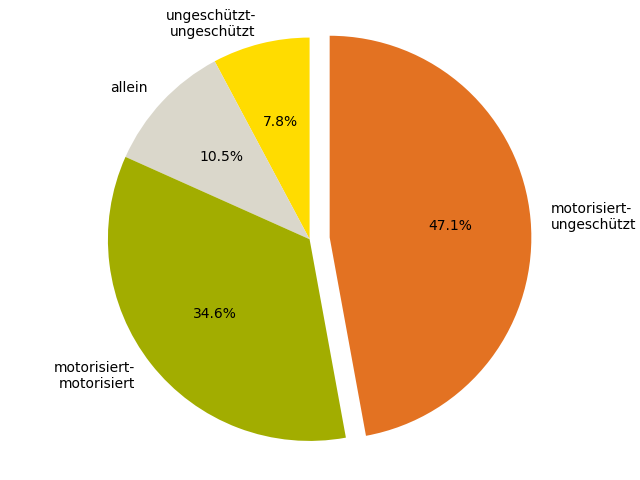
\includegraphics[width=8cm,height=6cm]{figures/motorisiert_ungeschuetzt}
		\caption[Beteiligung von motorisierrten und ungeschützten Verkehrsteilnehmern an Unfällen mit Personenschaden, die in den Jahren 2012 bis 2016 im Testgebiet aufgenommen wurden]{Beteiligung von motorisierrten und ungeschützten Verkehrsteilnehmern an Unfällen mit Personenschaden, die in den Jahren 2012 bis 2016 im Testgebiet aufgenommen wurden}\label{fig:Verkehrsbeteiligung_Personenschaden}
	\end{figure}
\end{savenotes}

In Abbildung \ref{fig:Verletzungsschwere_Pkw} ist die Verletzungsschwere von Pkw-Fahrer dargestellt. Andere motorisierte Verkehrsteilnehmer werden nicht betrachtet, da sie selten an Unfällen beteiligt sind (vgl. Abbildung \ref{fig:Beteiligungsart}). Pkw's sind zwar häufig an Unfällen mit Personenschaden beteiligt, tragen aber selbst selten eine Verletzung davon. Lediglich in 10\% der Unfälle mit Personenschaden wurde ein Pkw-Fahrer leicht verletzt.

\begin{savenotes}
	\begin{figure}[H]
		\centering
		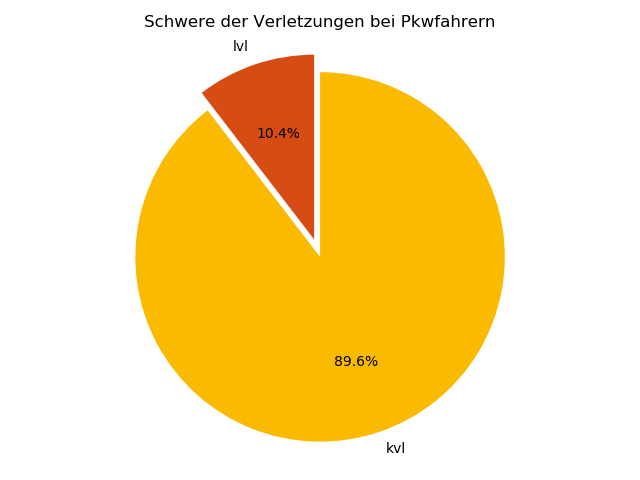
\includegraphics[width=8cm,height=6cm]{figures/Verl_Pkw}
		\caption[Schwere der Verletzungen von Pkw-Fahrern bei Unfällen mit Personenschaden, die in den Jahren 2012 bis 2016 im Testgebiet aufgenommen wurden ]{Schwere der Verletzungen von Pkw-Fahrern bei Unfällen mit Personenschaden, die in den Jahren 2012 bis 2016 im Testgebiet aufgenommen wurden}\label{fig:Verletzungsschwere_Pkw}
	\end{figure}
\end{savenotes}

Bei Radfahrern kommt es dagegen bei Unfällen mit Personenschaden in über 80\% der Fälle zu Verletzungen. In 10\% wurden Radfahrer sogar schwer verletzt. Fußgänger sind zwar seltener an Unfällen beteiligt, tragen dafür bei einer Unfallbeteiligung fast immer eine Verletzung davon. Im Untersuchungsgebiet kam es bei 93\% der Unfälle an denen Fußgänger beteiligt waren zu einem Personenschaden. 80\% führten zu einer leichten Verletzung bei ca. 7\% wurden die Fußgänger schwer oder tödlich verletzt. Abbildung \ref{fig:Verletzungsschwere_Rad_Fuss} stellt die Verletzungsschwere von Radfahrern und Fußgängern bei Unfällen mit Personenschaden dar. Die Annahmen in \textit{Hypothese 5}, dass der Verletzungsgrad bei Ungeschützten Verkehrsteilnehmern höher ist kann daher bestätigt werden. 

\begin{savenotes}
	\begin{figure}[H]
		\centering
		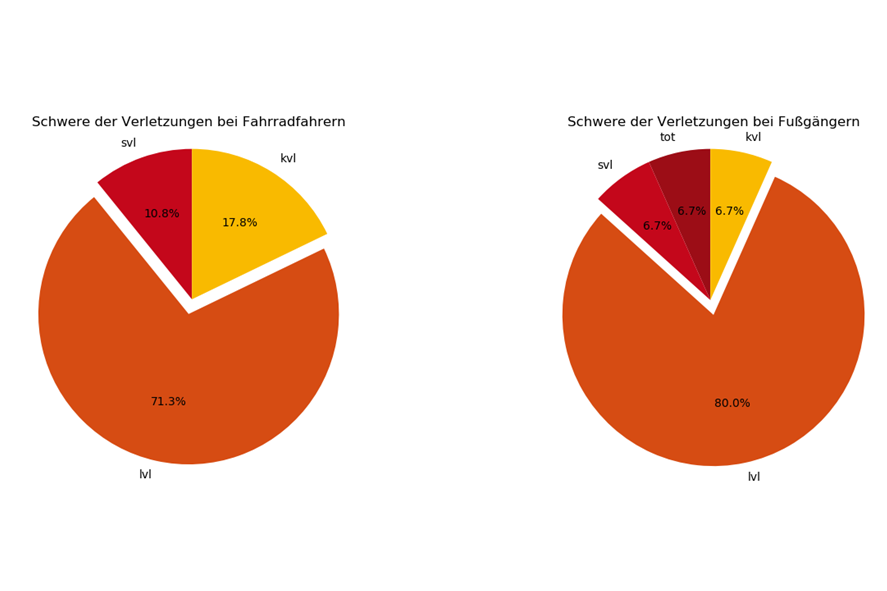
\includegraphics[width=11cm,height=6cm]{figures/Verl_Rad_Fuss}
		\caption[Schwere der Verletzungen von Radfahrern und Fußgängern bei Unfällen mit Personenschaden, die in den Jahren 2012 bis 2016 im Testgebiet aufgenommen wurden ]{Schwere der Verletzungen von Radfahrern und Fußgängern bei Unfällen mit Personenschaden, die in den Jahren 2012 bis 2016 im Testgebiet aufgenommen wurden}\label{fig:Verletzungsschwere_Rad_Fuss}
	\end{figure}
\end{savenotes}

\subsection{Unfälle mit Radfahrerbeteiligung beim Abbiegen}\label{subsection:Abbiegeunfälle mit Radfahrern}
Bei Unfällen bei denen die Unfallursache \enquote{Fehler beim Abbiegen nach rechts} (34) angegeben wurde kam es in 86\% der Fälle zu Unfällen mit Radfahrern. Dabei waren die Radfahrer, bis auf einmal, nicht Hauptverursacher der Unfalls. Bei den Hauptverursachern handelte es sich in fast 89\% der Fällen um Pkw-Fahrer. Bei drei Unfällen waren Lkw-Fahrer die Hauptverursacher, bei jeweils einem Unfall ein Motorrad- und ein Reisebusfahrer. Insgesamt kam es innerhalb des Testgebiets im Untersuchungszeitraum zu 45 Unfällen mit Radfahrerbeteiligung, bei denen die Ursache \enquote{Fehler beim Abbiegen nach rechts} bei den jeweiligen Hauptverursachern des Unfalls angegeben wurde.

\begin{savenotes}
	\begin{figure}[H]
		\centering
		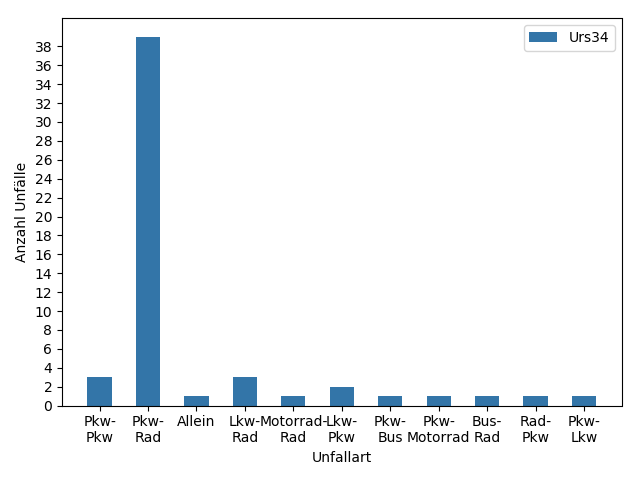
\includegraphics[width=8cm,height=6cm]{figures/Urs34_Beteiligung}
		\caption[Art der Verkehrsbeteiligung bei Unfällen mit der Unfallursache 34, die in den Jahren 2012 bis 2016 im Testgebiet aufgenommen wurden]{Art der Verkehrsbeteiligung bei Unfällen mit der Unfallursache 34, die in den Jahren 2012 bis 2016 im Testgebiet aufgenommen wurden}\label{fig:Urs34_Verkehrsbeteiligung}
	\end{figure}
\end{savenotes}

Die Ursache \enquote{Fehler beim Abbiegen nach links} (35) wurde lediglich bei ca. 26\% der Unfälle mit Radfahrerbeteiligung angegeben. Hierbei war keiner der Radfahrer Hauptverursacher. Bei den Hauptverursachern handelte es sich bis auf einen Fall, Motorradfahrer, immer um Pkw-Fahrer. Innerhalb des Testgebiets ereigneten sich zwölf Unfälle mit Radfahrerbeteiligung, bei denen die Unfallursache 35 bei Hauptverursacher angegeben wurde. Die Abbildungen \ref{fig:Urs34_Verkehrsbeteiligung} und \ref{fig:Urs35_Verkehrsbeteiligung} zeigen, bei wie vielen Unfällen im Testgebiet die zwei genannten Ursachen, mit den jeweiligen Unfallbeteiligten angegeben wurden. Auffällig ist, dass keine der beiden Ursachen bei Unfällen mit Fußgängern angegeben wurde.

\begin{savenotes}
	\begin{figure}[H]
		\centering
		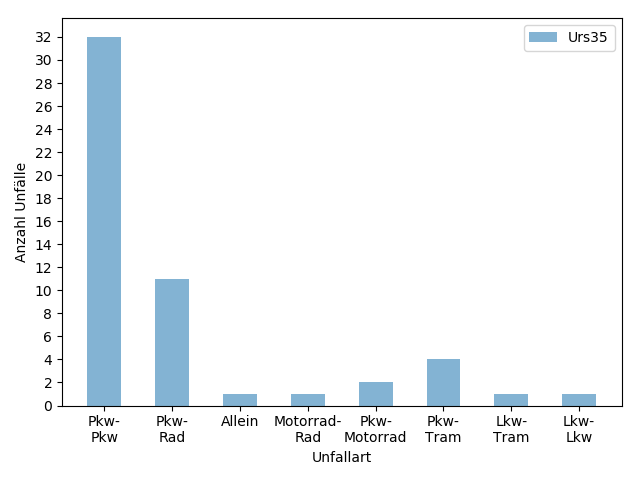
\includegraphics[width=8cm,height=6cm]{figures/Urs35_Beteiligung}
		\caption[Art der Verkehrsbeteiligung bei Unfällen mit der Unfallursache 35, die in den Jahren 2012 bis 2016 im Testgebiet aufgenommen wurden]{Art der Verkehrsbeteiligung bei Unfällen mit der Unfallursache 35, die in den Jahren 2012 bis 2016 im Testgebiet aufgenommen wurden}\label{fig:Urs35_Verkehrsbeteiligung}
	\end{figure}
\end{savenotes}

Betrachtet man die Unfallart, wurde bei den Unfällen mit der Ursache 34 und Radfahrerbeteiligung am häufigsten die Unfallart \enquote{Zusammenstoß mit Fahrzeug, das einbiegt oder kreuzt genannt} (5). Gefolgt von \enquote{Zusammenstoß mit Fahrzeug, das seitlich oder in gleiche Richtung fährt} (3) und \enquote{Zusammenstoß mit Fahrzeug, das entgegenkommt} (4). In einem Fall wurde die Ursache \enquote{Zusammenstoß mit Fahrzeug, anfährt, anhält, im ruh. Verkehr steht} (1) genannt. Wie in Abbildung \ref{fig:Unfallart_Urs34_Urs35_Radbeteiligung} zu erkennen ist, weisen die Unfälle mit der Unfallursache 35 ein ähnliches Bild auf. Hier steht lediglich die Unfallart 4 an zweiter und die Unfallart 3 an dritter Position .

\begin{savenotes}
	\begin{figure}[H]
		\centering
		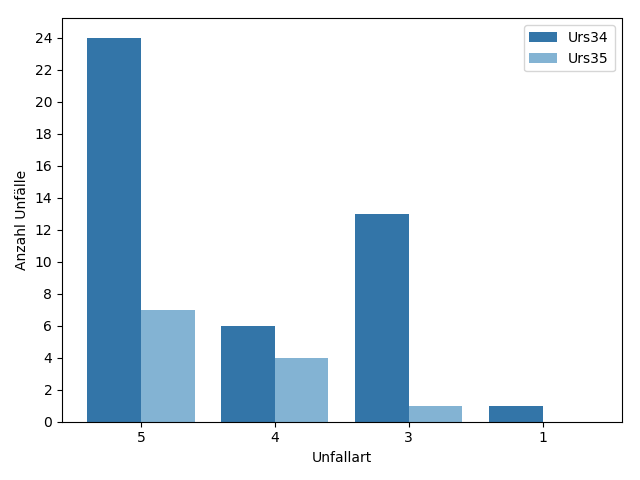
\includegraphics[width=8cm,height=6cm]{figures/Art_Urs34_Urs35}
		\caption[Unfallart bei Unfällen mit Radfahrerbeteiligung und Angabe der Unfallursache 34 bzw. 35, die in den Jahren 2012 bis 2016 im Testgebiet aufgenommen wurden]{Unfallart bei Unfällen mit Radfahrerbeteiligung und Angabe der Unfallursache 34 bzw. 35, die in den Jahren 2012 bis 2016 im Testgebiet aufgenommen wurden}\label{fig:Unfallart_Urs34_Urs35_Radbeteiligung}
	\end{figure}
\end{savenotes}

\textit{Hypothese 6} gibt an, dass sich beim Rechtsabbiegen häufiger Unfälle mit Radfahrern oder Fußgängern die sich parallel zum Fahrzeug bewegen ereignen als beim Linksabbiegen. Während sich deutlich mehr Unfälle mit Fahrradbeteiligung beim Rechtsabbiegen ereignen kann zu Unfällen mit Fußgängerbeteiligung anhand der vorhandenen Daten keine Angabe gemacht werden. Ob sich die Radfahrer bei den Unfällen parallel zum Unfallverursacher bewegt haben soll anhand der Unfallart überprüft werden. Wurde die Unfallart 3 oder 4 genannt, bewegten sich die Radfahrer parallel zum Unfallverursacher. Wurde die Unfallart 5 angegeben ist zunächst davon auszugehen, dass sich die Radfahrer hier nicht parallel zum Fahrzeugverkehr bewegten. Bei einer Stichprobenhaften Überprüfung der Kurzbeschreibungen für das Jahr 2013 bis 2016, ist zu erkennen, dass sich die Radfahrer auch hier häufig parallel zum Unfallverursacher bewegten. Da die Kurzbeschreibungen nicht für den gesamten Untersuchungszeitraum vorliegen soll hier zunächst nur darauf hingewiesen werden, dass auch Unfälle der Art 5 mit parallelen Bewegungen stattfinden können. Insgesamt wurde die Unfallart 5, wie in Abbildung \ref{fig:Unfallart_Urs34_Urs35_Radbeteiligung} zu erkennen ist, häufiger angegeben als Unfallart 3 und 4 zusammen. Die Annahme in \textit{Hypothese 6}, dass sich die Unfallbeteiligten parallel bewegten kann zunächst nicht bestätigt werden. Es sollte allerdings immer anhand der Kurzbeschreibungen überprüft werden, ob nicht auch Unfälle bei denen die Unfallart 5 genannt wurde solch ein Bewegungsmuster aufweisen.

Zusätzlich gibt \textit{Hypothese 6} an, dass kritische Situationen, vor allem dann entstehen, wenn Radfahrer den Radweg in die falsche Richtung befahren. Hierfür werden Unfälle mit Radfahrern im Untersuchungsgebiet betrachtet, bei denen die Ursachen \enquote{Verbotswidrige Benutzung der Fahrbahn oder anderer Straßenteile (z.B. Gehweg, Radweg)} (10) oder \enquote{Benutzung der Fahrbahn entgegen der vorgeschriebenen Fahrtrichtung in anderen Fällen} (9) angegeben wurden. Im Untersuchungszeitraum wurde bei insgesamt zwölf Unfällen mit Radfahrerbeteiligung die Ursache 10 angegeben. Bis auf einmal wurde sie immer dem beteiligten Radfahrer zugeordnet. Es kam sieben mal zu Unfällen mit Pkw-Rad Beteiligung, vier mal ereignete sich ein Unfall mit zwei Radfahrern und einmal kam es zu einem Unfall mit Rad-Pkw Beteiligung. Der Erstgenannte ist hierbei immer der Unfallverursacher. Die Unfallursache 9 wurden lediglich bei zwei Unfälle mit Radfahrerbeteiligung angegeben. Um diesen Teil der \textit{Hypothese 6} bestätigen zu können müsste zu den Ursachen 10 und 9 noch die Ursachen 34 oder 35 angegeben werden. Es kommt im Untersuchungsgebiet jedoch nur zu einem Unfall mit Radbeteiligung, bei dem sowohl die Ursache 10 als auch die Ursache 35 aufgenommen wurden. \textit{Hypothese 6} kann daher in diesem Punkt nicht bestätigt werden.

\begin{savenotes}
	\begin{figure}[H]
		\centering
		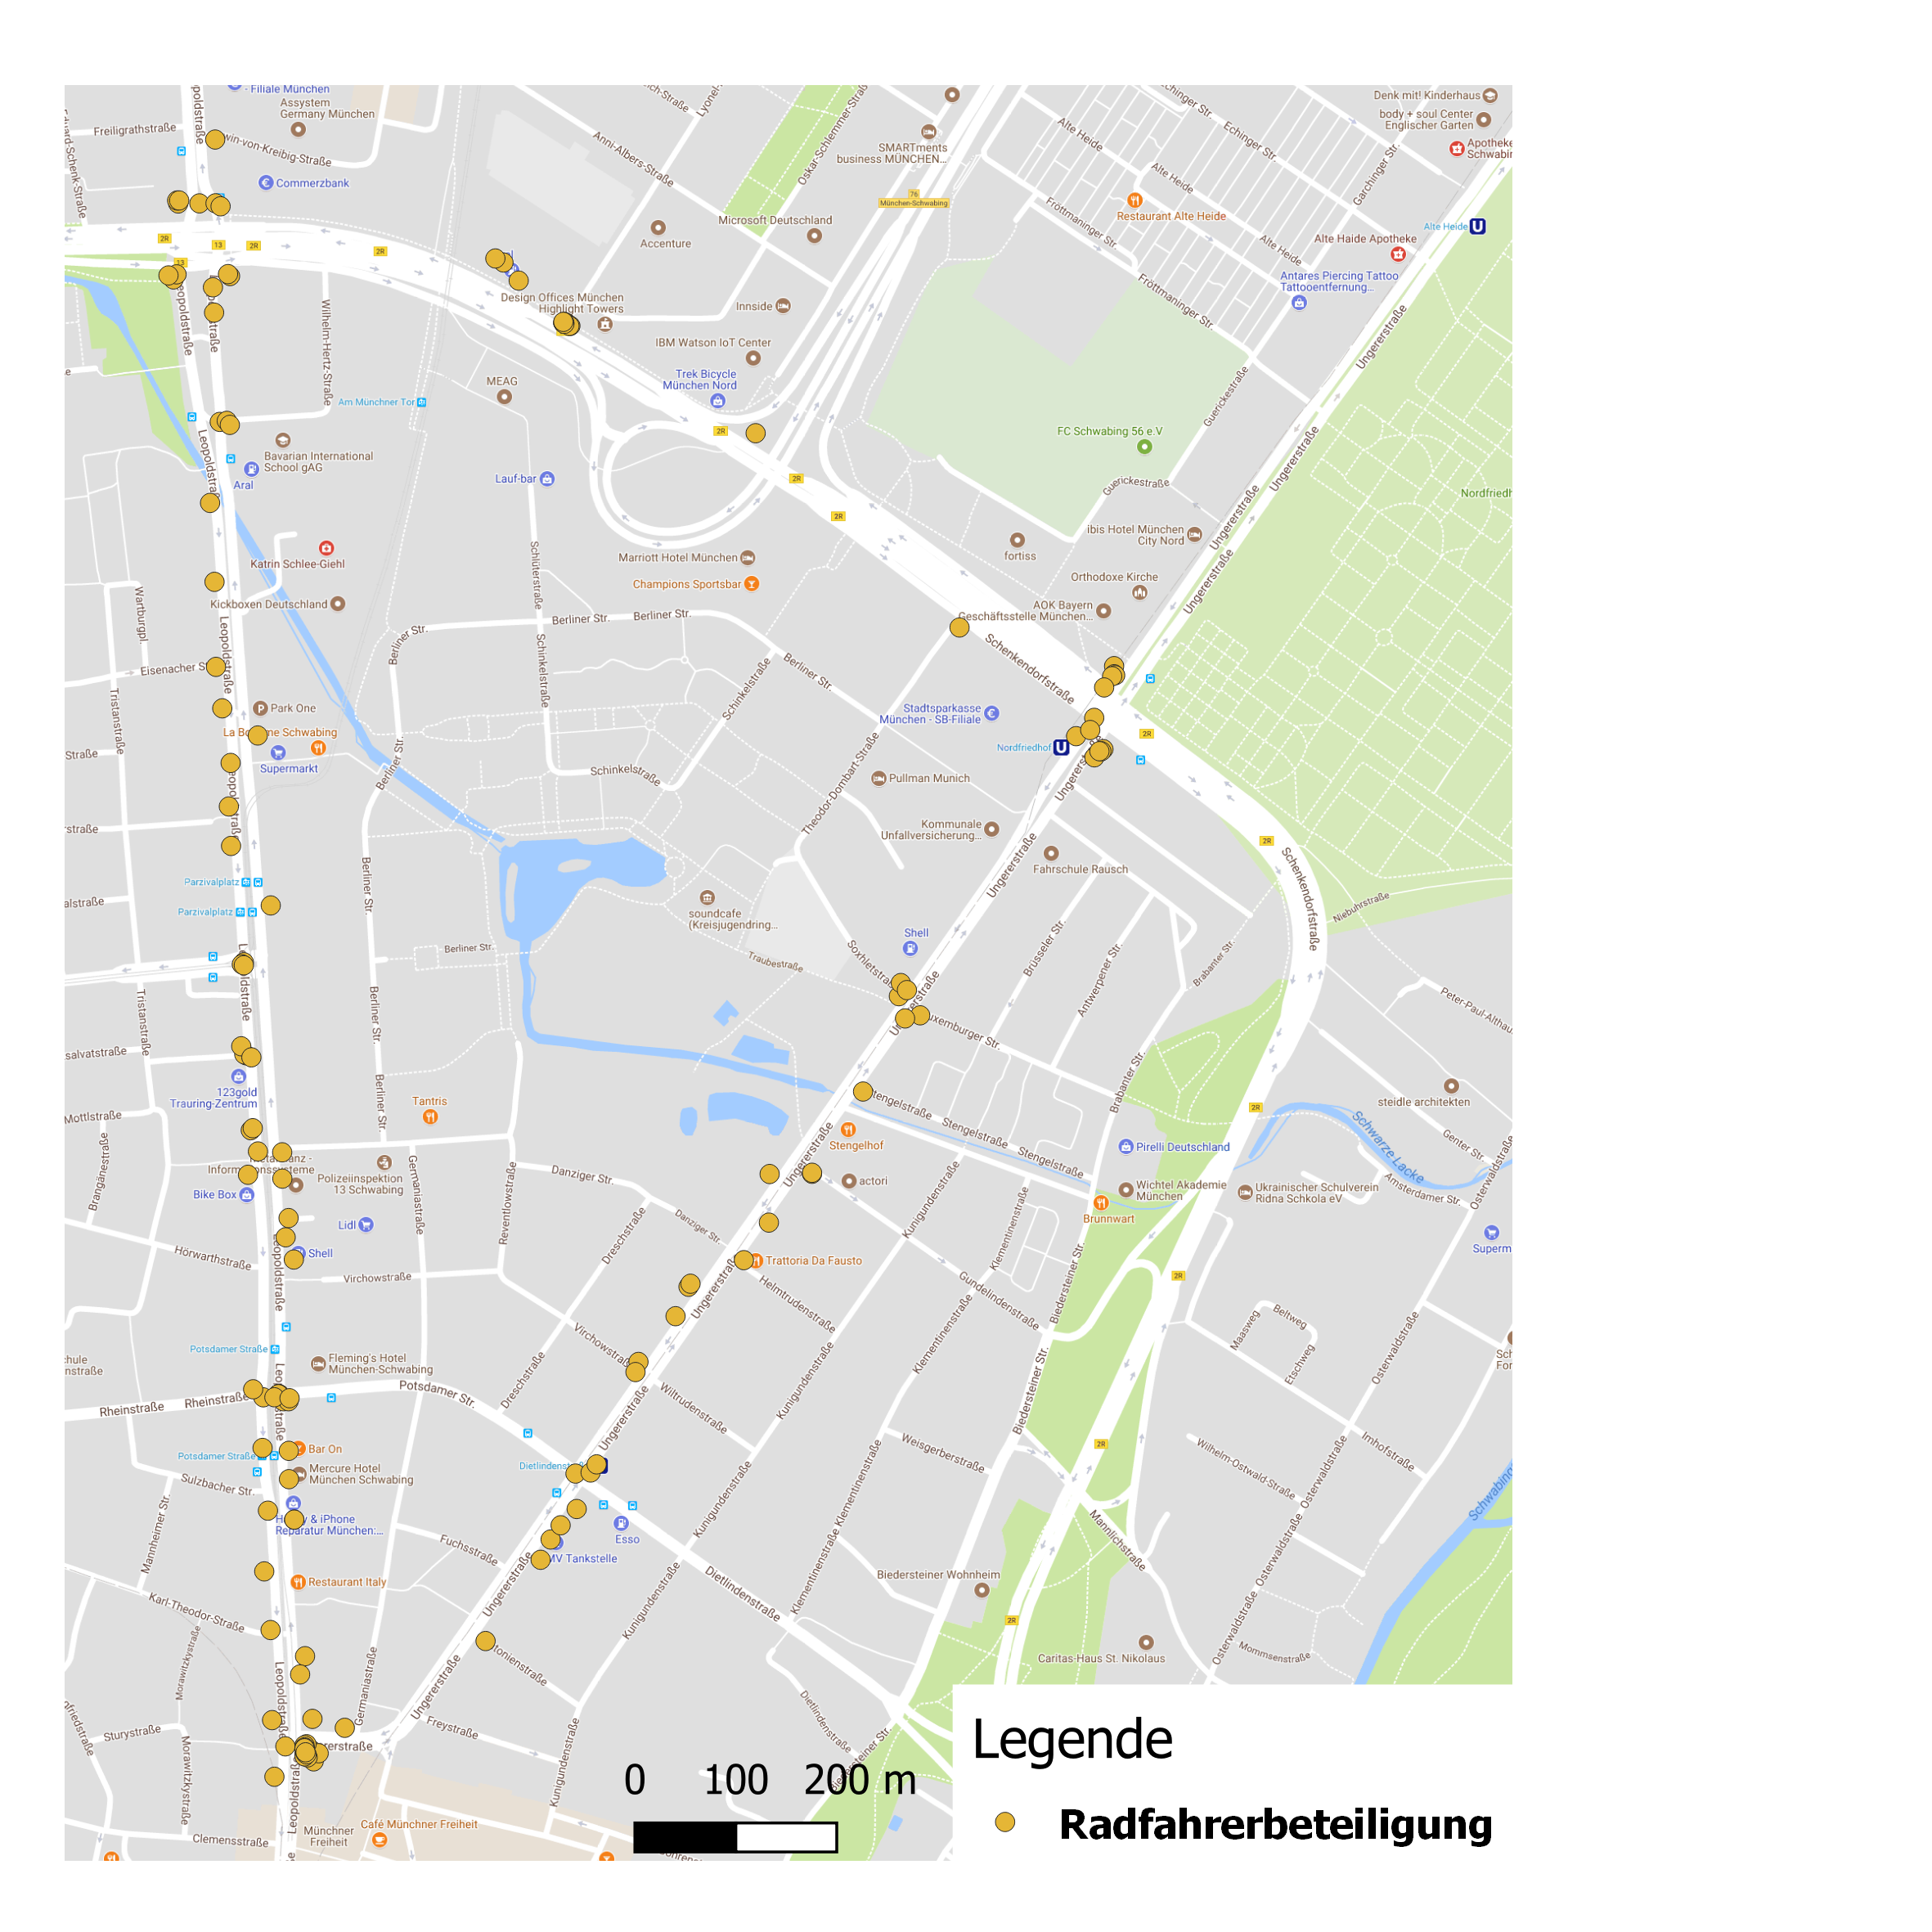
\includegraphics[width=10cm,height=10cm]{figures/map_radfahrer}
		\caption[Unfälle mit Fahrradbeteiligung, die in den Jahren 2012 bis 2016 im Testgebiet aufgenommen wurden]{Unfälle mit Fahrradbeteiligung, die in den Jahren 2012 bis 2016 im Testgebiet aufgenommen wurden}\label{fig:map_radfahrer}
	\end{figure}
\end{savenotes}

In Abbildung \ref{fig:map_radfahrer} werden die Unfälle mit Fahrradbeteiligung dargestellt. Hier ist zu erkennen, dass es an der Einmündung Leopoldstraße-Ungererstraße vermehrt zu Unfällen mit Fahrradfahrern kommt. Hierbei wurden x von y Unfällen durch Fehler beim Rechtsabbiegen ausgelöst. Hierbei kommt es vor allem zu Konflikten, wenn Fahrzeuge die Leopoldstraße in nördliche Richtung befahren und nach rechts auf die Ungererstraße abbiegen. Der Radweg darf hier in beide Richtungen befahren werden und ist im Bereich der Einmündung, zumindest im Konfliktbereich, rot Eingefärbt. Abbildung \ref{fig:Konflikt_Ungerer_Leo} wurde mit Blick in Richtung Norden aufgenommen, die Einfärbung ist rechts im Bild gut zu erkennen. Laut Bildern von Google Earth wurde die Markierung im Jahr 2016 angebracht. Das die vorhanden Unfalldaten nur bis zum Jahr 2016 reichen, kann nicht gesagt werden, ob die Konflikte reduziert werden konnten.

%Bei Gelegenheit noch ein besseres Bild machen!!
\begin{savenotes}
	\begin{figure}[H]
		\centering
		\includegraphics[width=8cm,height=6cm]{figures/Ungerer_Leo}
		\caption[Konfliktpunkt an der Einmündung Leopoldstrße-Ungererstraße mit eingefärbter Radverkehrsanlage]{Konfliktpunkt an der Einmündung Leopoldstrße-Ungererstraße mit eingefärbter Radverkehrsanlage}\label{fig:Konflikt_Ungerer_Leo}
	\end{figure}
\end{savenotes}

\subsection{Fehlverhalten der Fußgänger}
Um Fehlern von Fahrzeugführern und Fußgängern unterscheiden zu können gibt es Unfallursachen die das Falsche Verhalten der Fußgänger beschreiben. In Abbildung \ref{fig:Fehlverhalten_Fussgaenger} ist zu erkennen, dass im Testgebiet die Ursache \enquote{ohne auf den Fzg.-verkehr zu achten} (64) am häufigsten angegeben wurde. Hierbei kam es fast immer zu einem Unfall mit Personenschaden.

An zweiter Position steht die Ursache \enquote{andere Fehler der Fußgänger} (69). Obwohl es bei sechs Unfällen einen Personenschaden gab wurden keine weiteren Angaben gemacht um was für Fehler es sich genau handelt. Währen es sich bei der erst genannten Unfallursache meist um Situationen handelt, in denen Fußgänger einfach auf die Straße treten ohne den Fzg.-Verkehr zu beachten kann dieser Punkt keiner bestimmten Situation im Straßenraum zugeordnet werden. Weitere Unfälle ereigneten sich \enquote{durch plötzliches Hervortreten hinter Sichthindernissen} (63), \enquote{in der Nähe von Kreuzungen oder Einmündungen, Lichtzeichenanlagen oder Fußgängerüberwegen, bei dichtem Verkehr an anderen Stellen} (62) oder durch \enquote{Nichtbenutzen des Gehwegs} (65). Wenn diese drei Unfallursachen angegeben wurden kam es in acht von zehn Fällen zu einem Personenschaden. Etwas seltener und mit geringeren Folgen wurden dagegen die Ursachen \enquote{Nichtbenutzen der vorgeschrieben Straßenseite} (67) und \enquote{Nichtbenutzen des Gehwegs} (66) angegeben.

\begin{savenotes}
	\begin{figure}[H]
		\centering
		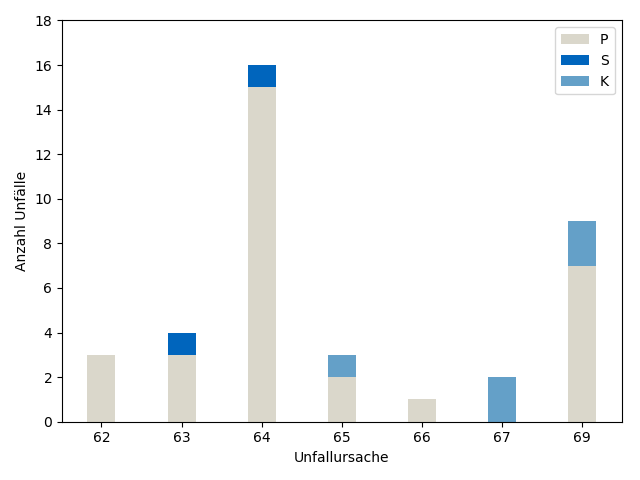
\includegraphics[width=8cm,height=6cm]{figures/Urs_Fussgaenger}
		\caption[Unfallursachen durch falsches Verhalten der Fußgänger mit zugehörigem Unfallmodus, die bei Unfällen in den Jahren 2012 bis 2016 im Testgebiet angegeben wurden]{Unfallursachen durch falsches Verhalten der Fußgänger mit zugehörigem Unfallmodus, die bei Unfällen in den Jahren 2012 bis 2016 im Testgebiet angegeben wurden}\label{fig:Fehlverhalten_Fussgaenger}
	\end{figure}
\end{savenotes}

In Abbildung \ref{fig:Beteiligungsart} ist zu erkennen, dass bei etwas mehr als der Hälfte der Unfälle mit Fußgängerbeteiligung, Fußgänger selbst die Hauptverursacher sind. Betrachtet man hier nochmals die Unfallursache \enquote{ohne auf den Fzg.-verkehr zu achten} wurden sogar bei ca. 81\% der Unfälle Fußgänger als Hauptbeteiligter angegeben. \textit{Hypothese 8} gibt an, dass Falsches Verhalten der Fußgänger häufig die Ursache für Unfälle mit Personenschaden im urbanen Raum ist. Im Vergleich zu Kfz sind Fußgänger zwar seltener an Unfällen beteiligt, dafür kommt es bei einer Beteiligung häufig zu Personenschaden. Im Testgebiet gab es innerhalb von fünf Jahren 36 Unfälle mit Fußgängerbeteiligung, dabei kam es bei 30 zu einem Personenschaden. Betrachtet man alle Unfälle mit Personenschaden im Untersuchungsgebiet wurde immerhin bei 10\% der Unfälle als Unfallursache falsches Verhalten der Fußgänger angegeben. \textit{Hypothese 8} kann daher in diesem Punkt bestätigt werden.

Zusätzlich wurde in \textit{Hypothese 8} angenommen, dass die Unfallursachen Rotlichtverstöße (60) und \enquote{Überschreiten der Fahrbahn ohne auf den Fzg.-verkehr zu achten} dabei am häufigsten auftreten. In Abbildung \ref{fig:Fehlverhalten_Fussgaenger} ist zu erkennen, dass Rotlichtverstöße innerhalb von fünf Jahren im Untersuchungsgebiet gar nicht aufgenommen wurden, während \enquote{Überschreiten der Fahrbahn ohne auf den Fzg.-verkehr zu achten} am häufigsten genannt wurde. Abbildung \ref{fig:Verletzungen_Urs64} bezieht sich nur auf diese Ursache und gibt die Schwere der Verletzungen an. Hierbei ist auffällig, dass es lediglich bei 12,5\% der am Unfall Beteiligten keine Verletzung (kvl) auftrat. Bei über 60\% kam es zu leichten Verletzungen (lvl) und in jeweils 12,5\% der Fälle wurden Unfallbeteiligte schwer (svl) oder sogar tödlich Verletzt (tot). Eine tödlich Verletzung trat im gesamten Untersuchungsgebiet innerhalb der Untersuchungszeitraums nur bei zwei Unfällen auf, diese machen genau die eben genannten 12,5\% der Unfallursache 64 aus. Die \textit{Hypothese 8} kann zwar in ihrem zweiten Teil nur in einem Punkt bestätigt werden. Dieser hat dafür einen wesentlichen Einfluss auf Unfälle mit Personenschaden.

\begin{savenotes}
	\begin{figure}[H]
		\centering
		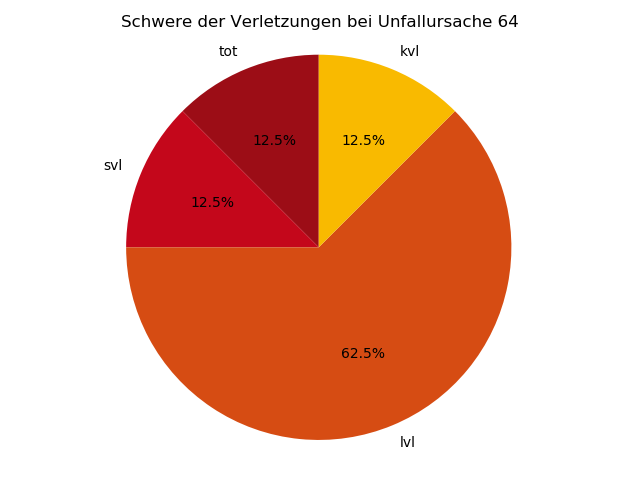
\includegraphics[width=8cm,height=6cm]{figures/Urs64}
		\caption[Verletzungen die durch Unfälle mit Angabe der Ursache 64 bei Unfällen in den Jahren 2012 bis 2016 im Testgebiet angegeben wurden]{Verletzungen die durch Unfälle mit Angabe der Ursache 64 bei Unfällen in den Jahren 2012 bis 2016 im Testgebiet angegeben wurdenn}\label{fig:Verletzungen_Urs64}
	\end{figure}
\end{savenotes}


Betrachtetet man die den Unfällen mit Fußgängerbeteiligung zugeordneten Besonderheit wurden im Testgebiet nur vier Mal \enquote{Fußgängerfurt} und sechs Mal \enquote{Haltestelle} angegeben. Überraschend ist, dass es bei \enquote{Fußgängerüberwegen} kein Unfall mit Fußgängern gab. Obwohl diese Besonderheit in Abbildung \ref{fig:BES} am häufigstten vorkommt. In \textit{Hypothese 8} wird vermutet, dass sich Unfälle mit Fußgängern häufig in der Nähe von ÖPNV Haltestellen ereignen.

\begin{savenotes}
	\begin{figure}[H]
		\centering
		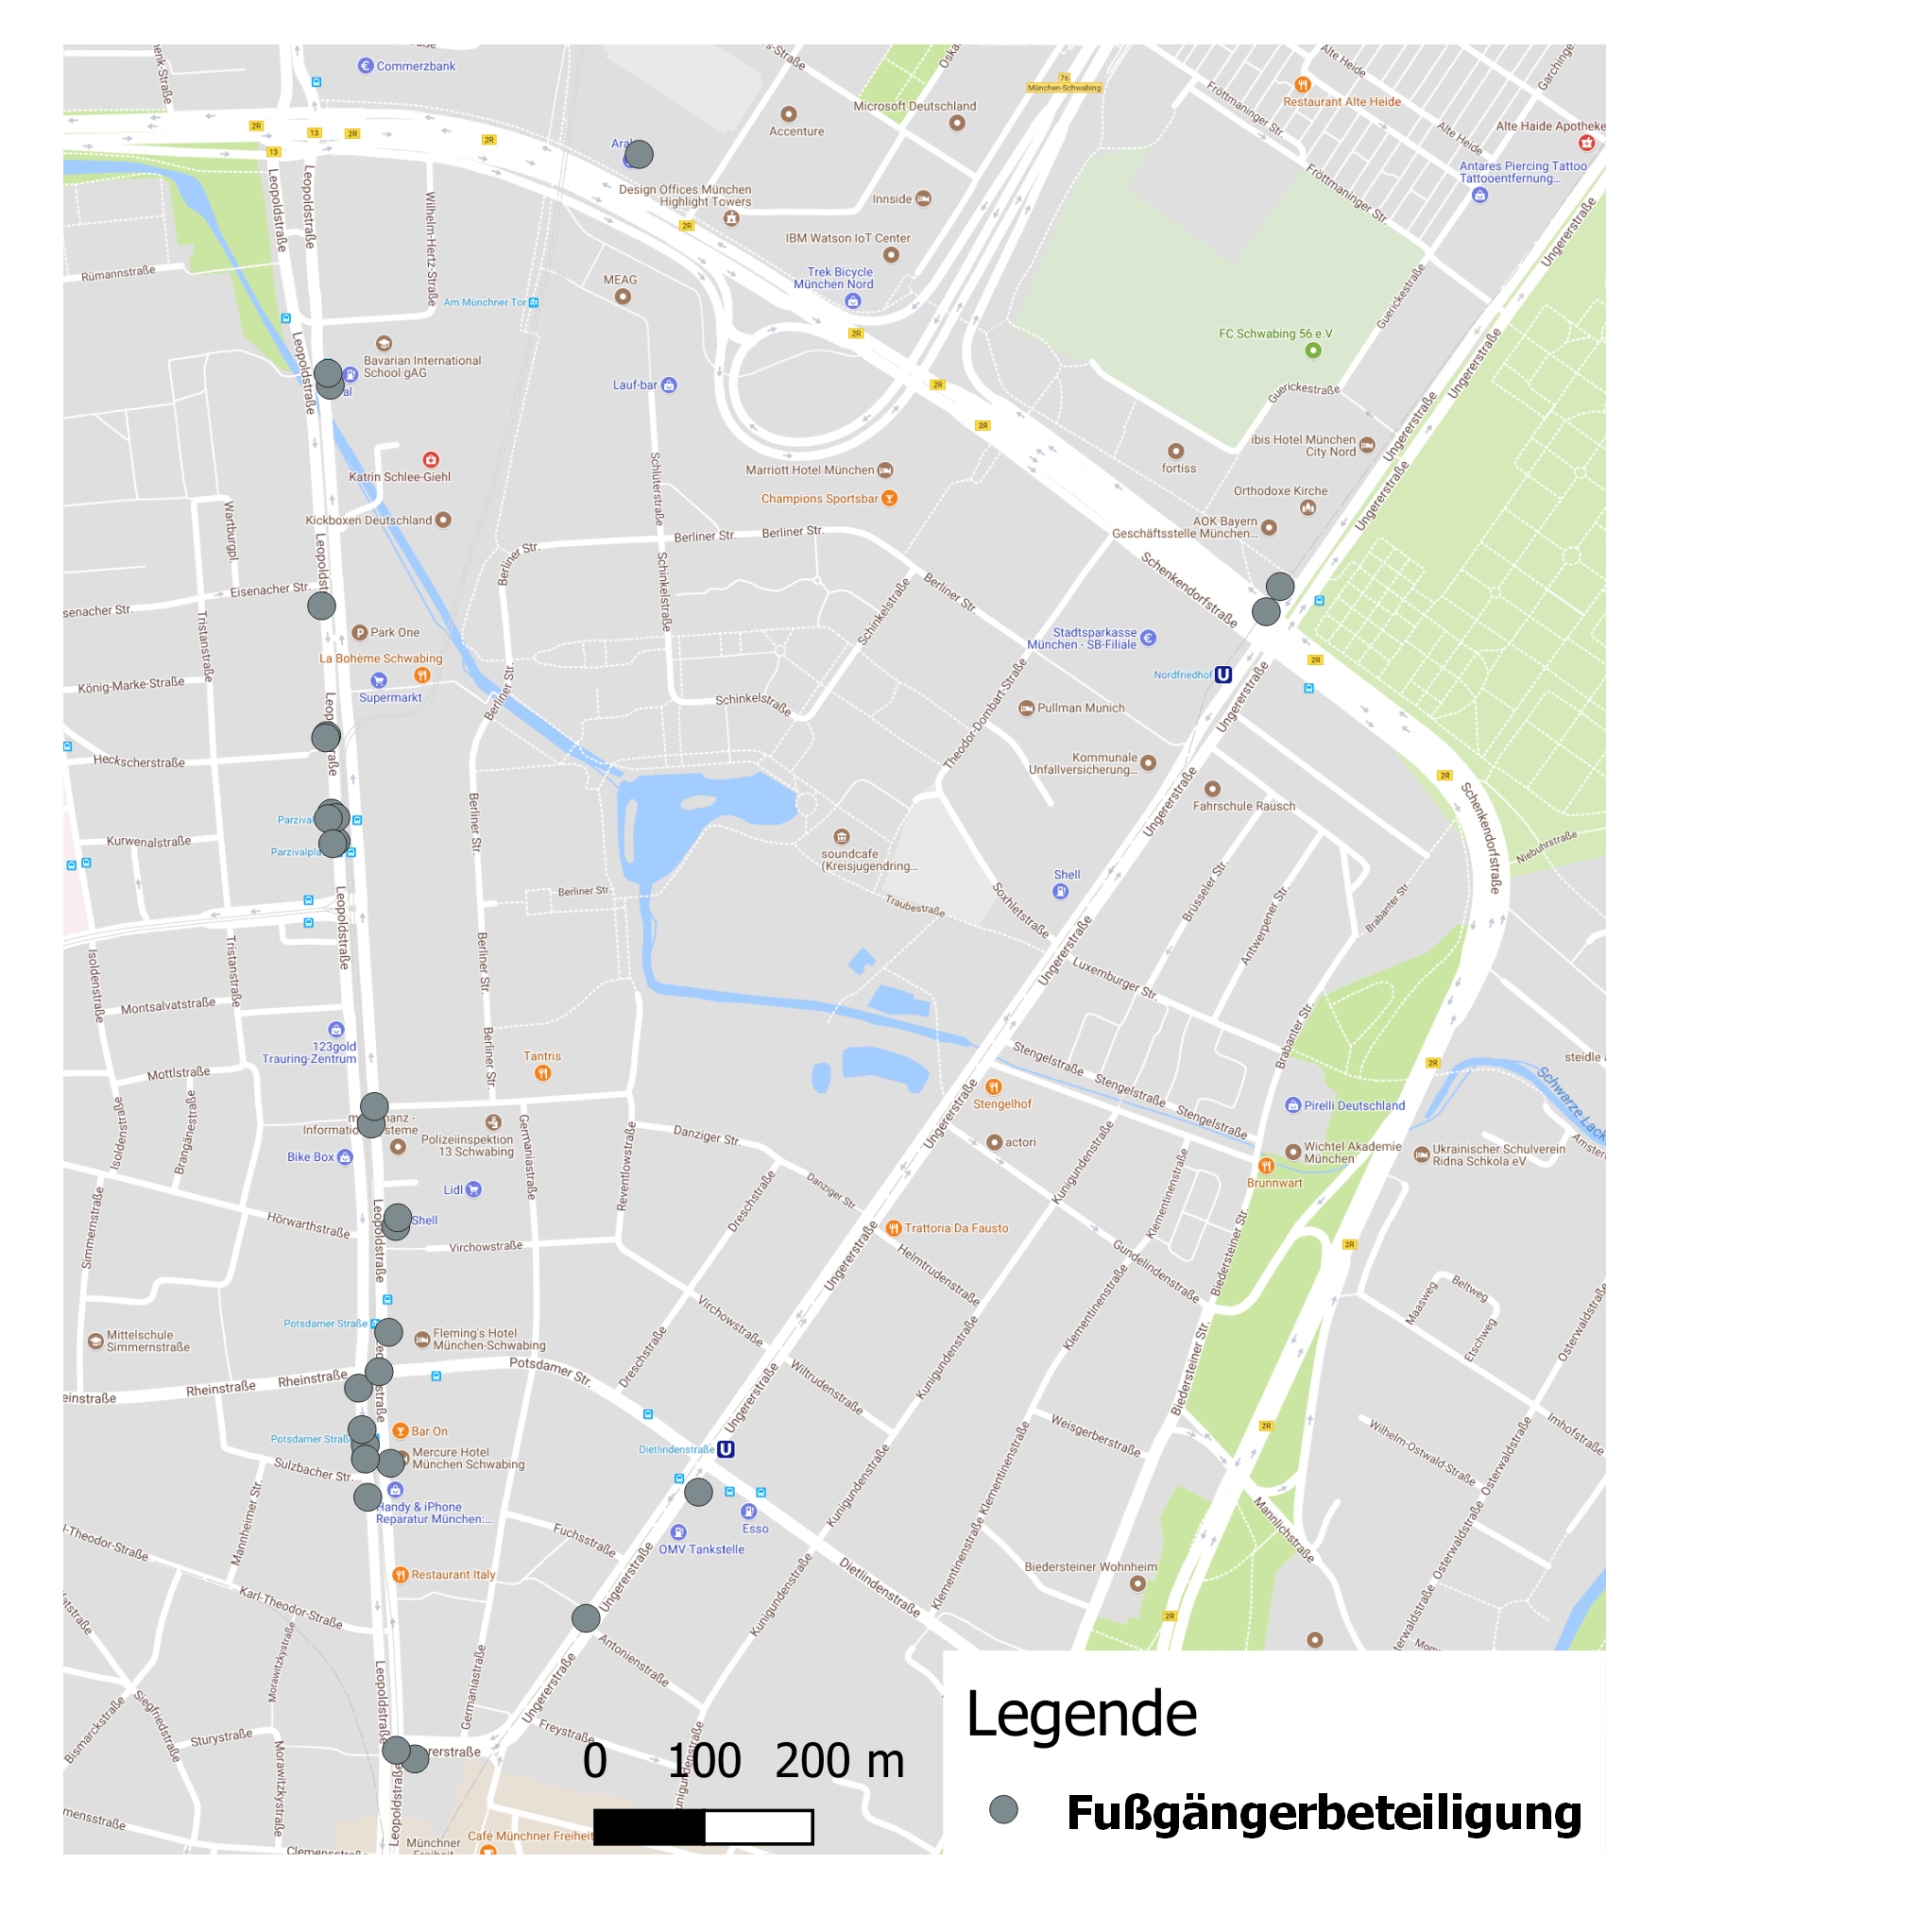
\includegraphics[width=10cm,height=10cm]{figures/map_fussgaenger}
		\caption[Unfälle mit Fußgängerbeteiligung, die in den Jahren 2012 bis 2016 im Testgebiet aufgenommen wurden]{Unfälle mit Fußgängerbeteiligung, die in den Jahren 2012 bis 2016 im Testgebiet aufgenommen wurden}\label{fig:map_fussganeger}
	\end{figure}
\end{savenotes}

Betrachtet man Abbildung \ref{fig:map_fussganeger} ist zu erkenne, dass sich vor allem im Bereich der Haltestellen Parzivalplatz und Potsdamer Straße Unfälle ereigneten. Am Parzivalplatz ereigneten sich fast 17\% der Unfälle mit Fußgängerbeteiligung um Bereich der Haltestelle Potsdamer Straße sogar 23\%. Die beiden tödlichen Unfälle im Untersuchungszeitraum traten jeweils an einer der Haltestellen auf. \textit{Hypothese 8} kann somit in diesem Punkt bestätigt werden. Auffällig ist auch, dass alle, bis auf fünf, Unfälle bei denen Fußgänger beteiligt waren auf der Leopoldstraße aufgenommen wurden.

\subsection{Besonderheiten der Unfallstelle}
Besonderheiten der Unfallstelle werden nur bei Unfällen mit Personen- und Sachschaden angegeben. Innerhalb des Testgebiets wurden in fünf Jahren bei 11,9\% der Unfälle mit Personenschaden und bei lediglich 3,7\% mit Sachschaden Besonderheiten angegeben. In Abbildung \ref{fig:BES} werden die angegebenen Besonderheiten mit zugehörigem Unfallmodus dargestellt. Am häufigsten wurde als Besonderheit \enquote{Fußgängerüberweg} (3) angegeben. Gefolgt von \enquote{Fußgängerfurt} (4) und \enquote{Haltestelle} (5). Betrachtet man diese drei Punkte genauer, fällt auf dass es bei Unfällen an denen die Besonderheit Haltestelle genannt wurde am häufigsten zu Unfällen mit Personenschaden kommt. Unfälle an Fußgängerfurten führen ebenfalls häufiger zu Personen- als zu Sachschaden, während bei Fußgängerüberwegen die Unfälle mit Sachschaden überwiegen. Neben Fußgängerüberweg gibt es noch den \enquote{Schienengleichen Wegübergang} (2). Diese Besonderheit wurde im Untersuchungsgebiet nur in zwei Fällen angegeben. Hierbei muss darauf hingewiesen werden, dass diese Eigenschaft nur in der Leopoldstraße, in dem Bereich mit Tram, angegeben werden kann.

In lediglich einem Fall wurde \enquote{Unübersichtlich} (1) als Besonderheit angegeben und in drei Fällen war eine \enquote{Arbeitsstelle} (6) im Bereich des Unfallorts vorhanden. Da sich innerhalb der Teststrecke kein Verkehrsberuhigter Bereich befindet, wurde diese Besonderheit (7) auch nie angegeben. 

\begin{savenotes}
	\begin{figure}[H]
		\centering
		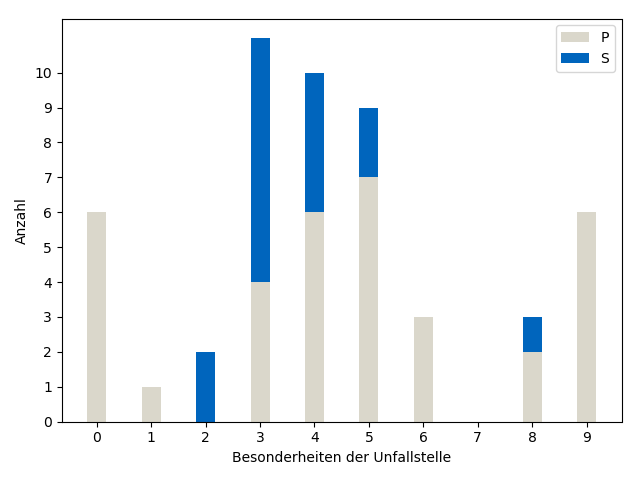
\includegraphics[width=8cm,height=6cm]{figures/BES}
		\caption[Besonderheiten der Unfallstelle mit zugehörigem Unfallmodus, die bei Unfällen in den Jahren 2012 bis 2016 im Testgebiet angegeben wurden]{Besonderheiten der Unfallstellen mit zugehörigem Unfallmodus, die bei Unfällen in den Jahren 2012 bis 2016 im Testgebiet angegeben wurden}\label{fig:BES}
	\end{figure}
\end{savenotes}

Bei Unfälle mit Personenschaden wurden die Besonderheiten \enquote{Benutzungspflicht der Radverkehrsanlage} (0) und \enquote{baulich von der Fahrbahn getrennte Radverkehrsanlage} am zweithäufigsten angegeben. Auffällig ist, dass diese Besonderheiten nur bei Unfällen mit Personenschaden angegeben wurden. /{Radverkehrsanlagen auf der Fahrbahn oder lediglich durch Markierung von der Fahrbahn abgetrennt} (8) wurde im Vergleich zu den zwei vorherigen Besonderheiten seltener angegeben. Während die Besonderheiten 7 und 9 jeweils 2\% der Unfällen mit Personenschaden ausmachen wurde 8 nur in 0,8\% der Fälle genannt.

\textit{Hypothese 7} gibt an, dass es bei baulich getrennten Radverkehrsanlagen häufiger zu Unfällen kommt als bei Radverkehrsanlagen auf der Fahrbahn. Die Anzahl der Unfälle bei denen diese zwei Punkte als Besonderheit genannt wurden ist zwar gering, trotzdem ist in Abbildung \ref{fig:BES} zu erkennen, dass es bei baulich getrennten Radverkehrsanlagen häufiger zu Unfällen  kam. Hierbei muss jedoch beachtet werden, dass innerhalb des Testgebiets größtenteils nur solche Radverkehrsanlagen vorhanden sind. Betrachtet man diese zwei Besonderheiten etwas genauer fällt auf, dass die Radfahrer ungefähr zu gleichen Teilen als Beteiligter01 und Beteiligter02 angegeben werden. Zudem kommt es auf baulich getrennten Radverkehrsanlagen häufig zu Unfällen zwischen zwei Radfahrern oder zwischen Fahrrad und Fußgänger bzw. Fahrrad und Moped. Die Unfälle bei denen angegeben wurde, dass es sich um Radverkehrsanlagen auf der Fahrbahn handelt wiesen alle einen Konflikt zwischen Pkw und Fahrrad auf.

Im Testgebiet traten an der Einmündung Schenkendorfstraße/Leyonel-Feininger-Straße häufig Unfälle mit Fahrradbeteiligung auf siehe Abbildung %xy. (Karte mit Unfallschwerpunkt/evtl. Karte nach Art der Beteiligung erstellen?) Evtl. Adrian zitieren, hat das auch schon festgestellt. Allerdings nur Einbiegeunfall.
Hierbei wurde bei zwei Unfällen die Besonderheit Radverkehrsanlage auf der Straße und bei einem getrennte Radverkehrsanlage angegeben. Bei den ersten zwei Unfällen ereignete sich der Unfall direkt am Knotenpunkt. Es kam dabei jeweils zu einem Unfall zwischen einem Pkw der nach rechts auf die Schenkendorfstraße einbiegen wollte und einem Radfahrer der von rechts kam. Der Radweg darf an dieser Stelle in beide Richtungen befahren werden. Der dritte Unfall trat an der Tankstelle unmittelbar neben der Einmündung auf. Auch hier wollte ein Pkw nach rechts Einbiegen und übersah einen von rechts kommenden Radfahrer. Da dieser Unfall sich allerdings im Bereich der Tankstelle ereignete wurde getrennte Radverkehrsanlage als Besonderheit angegeben. Die beiden Stelle sind im Abbildung \ref{fig:Lyonel-Feininger} zu erkennen. In diesem Fall ist nicht die Art der Radverkehrsanlage für die Unfallhäufungen verantwortlich, sondern die Freigabe des Radwegs entgegen die Fahrtrichtung. Mit dieser Situation rechnen Fahrzeugführer häufig nicht, obwohl an der Einmündung, vgl. Abbildung \ref{fig:Lyonel-Feininger}, deutlich kenntlich gemacht wurde, dass Radfahrer von beiden Seiten kommen können. Die Markierungen waren laut Bildern von Google Earth auch schon zu den jeweiligen Unfallzeitpunkten vorhanden.

\begin{savenotes}
	\begin{figure}[H]
		\centering
		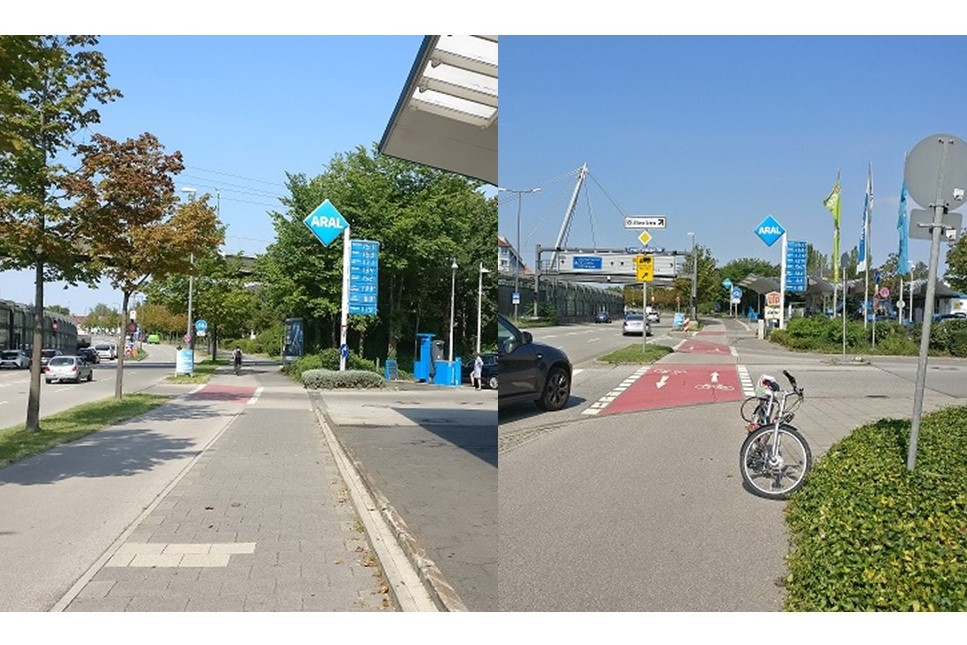
\includegraphics[width=12cm,height=8cm]{figures/Lyonel_Feininger}
		\caption[Ausfahrt Aral Tankstelle und Einmündung Lyonel-Feininger-Straße]{Links: Ausfahrt der Aral Tankstelle mit baulich von der Fahrbahn getrennter Radverkehrsanlage Rechts: Einmündung mit markiertem Radweg auf der Fahrbahn}\label{fig:Lyonel-Feininger}
	\end{figure}
\end{savenotes}

\textit{Hypothese 7} kann daher nur bedingt bestätigt werden. Sie wird zunächst Anhand der statistischen Auswertung in Abbildung \ref{fig:BES} bekräftigt. Das Unfallgeschehen an der Einmündung Lyonel-Feininger-Straße macht dagegen deutlich, dass nicht nur die Art der Radverkehrsanlage sondern auch die Führung der Radfahrer von Bedeutung ist. Zusätzlich scheint der Einfluss der vorhanden Markierung, trotz Roteinfärbung, nicht den gewünschten Effet zu erbringen. Dies kann jedoch nicht nachgewiesen werden, da keine Unfallzahlen für einen Zeitraum vorliegen, in dem keine Markierung vorhanden war. 

%Statistischer Test um Aussagekraft zu belegen?

\subsection{Einfluss allgemeiner Unfallursachen}
Neben den persönlichen Ursachen können je Unfall bis zu zwei allgemeine Ursachen angegeben werden. Abbildung \ref{fig:allg_Ursachen} zeigt die allgemeinen Ursachen die Unfällen im Testgebiet innerhalb von fünf Jahren zugewiesen wurden. Es ist zu erkennen, dass \enquote{Glätte oder Schlüpfrigkeit der Fahrbahn} (Nr. 70 bis 74) neben dem Punkt \enquote{Sonstige Ursachen} (Nr. 89) am häufigsten zu Unfällen führten. Obwohl sonstige Ursachen am häufigsten genannt wurden, können sie hier nicht näher betrachtet werden, da keine zusätzlichen Beschreibungen über die Art vorliegen. Auffällig ist, dass Schnee, Eis (Nr. 72) zwar häufiger als Unfallursache angegeben wurden, Regen (Nr. 72) dafür zu mehr Unfällen mit Personenschaden führt. 

\begin{savenotes}
	\begin{figure}[H]
		\centering
		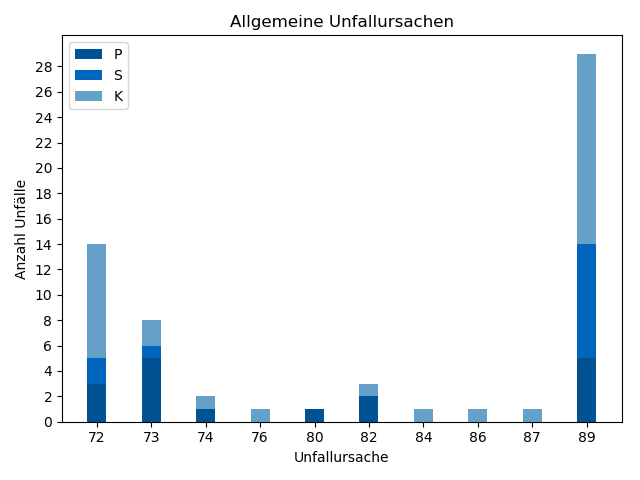
\includegraphics[width=8cm,height=6cm]{figures/allg_Ursachen}
		\caption[Allgemeinen Unfallursachen mit Unfallmodus, die bei Unfällen in den Jahren 2012 bis 2016 im Testgebiet angegeben wurden]{[Allgemeinen Unfallursachen mit Unfallmodus, die bei Unfällen in den Jahren 2012 bis 2016 im Testgebiet angegeben wurden}\label{fig:allg_Ursachen}
	\end{figure}
\end{savenotes}

Witterungseinflüsse können nicht nur die Straßenverhältnisse beeinflussen sondern auch zu Sichtbehinderungen führen (Nr. 80 bis 84). Innerhalb von fünf Jahren wurden im Testgebiet jedoch nur bei fünf Unfällen eine dieser Ursachen angegeben. Jeweils ein Unfall wurde durch starken Regen, Hagel, Schnee (Nr. 81) bzw. Unwetter (Nr. 84) und drei durch blendende Sonne (Nr. 82) beeinflusst. Zwei der Unfälle die sich durch Sonnenblendung ereigneten hatten sogar einen Personenschaden zur Folge. Betrachtete man jedoch alle Unfälle mit Personenschaden im Untersuchungsgebiet über die fünf Jahre wurden lediglich 0,7 \% durch blendende Sonne beeinflusst. \textit{Hypothese 9} gibt an, dass es bei Sichtbehinderung durch blendende Sonne vermehrt zu Unfällen kommt. Blendende Sonne wird zwar im Vergleich zu den anderen Ursachen am häufigsten genannt, aber trotzdem zu selten um ihr eine wirkliche Bedeutung zukommen zu lasse. \textit{Hypothese 9} kann daher nicht bestätigt werden. %Kann man das einfach so schreiben?
Trotzdem sollte man die Einwirkung durch blendende Sonne mit Fokus auf Kapitel \ref{chapter:automatisiertes Fahren} nicht vernachlässigen, Sensoren von automatisierten Fahrzeugen könnten hier Schwierigkeiten haben.
 
Noch seltener haben der \enquote{Zustand der Straße} (Nr.75 bis 79) und \enquote{Hindernisse} Einfluss auf Unfälle innerhalb des Testgebiets. Sie werden im Summe nur drei mal genannt und deshalb nicht näher betrachtet. Allgemeine Unfallursachen, die in dem betrachteten Zeitraum nie einem Unfall zugewiesen wurden werden in Abbildung \ref{fig:allg_Ursachen} nicht berücksichtigt.

%Allg Fazit?

\section{Bewertung der Unfälle im Testgebiet}
Anhand der Bewertungsmethodik die in Kapitel \ref{section:Bewertung urbaner Fahrsituationen} vorgestellt wird werden die betrachteten Unfälle nun bezüglich ihrer Kritikalität bewertet. Hierfür werden zunächst nur die Unfälle betrachtet denen bei der Unfallaufnahme bereits ein Unfalltyp zugeordnet wurde. Anschließend werden alle Unfälle typisiert um die Unfallabläufe besser verstehen zu können. Bei der Bewertung der typisierten Unfälle werden so auch die Kleinunfälle berücksichtigt. Es werden zuerst nur die sieben Unfalltypen betrachtet und dann die jeweiligen Feintypen.

\subsection{Bewertung der Unfälle mit zugeordnetem Unfalltyp}
Betrachtet man nur die Unfälle, denen bereits bei der Unfallaufnahme ein Unfalltyp zugeordnet wurde, werden die Kleinunfälle nicht berücksichtigt und die Gesamtanzahl der Unfälle beträgt lediglich 591 Stück. In Abbildung \ref{fig:Bewertung_UT} werden all diese Unfälle anhand des Unfalltyps, der Unfallschwere und der aufgetretenen Häufigkeit dargestellt. Es ist zu erkennen, dass zwei Unfalltypen ein erhöhtes Risiko aufweisen.

\begin{savenotes}
	\begin{figure}[H]
		\centering
		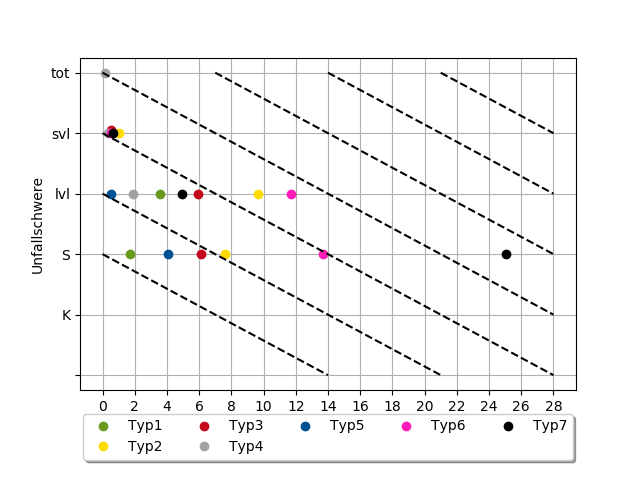
\includegraphics[width=12cm,height=8cm]{figures/Bewertung_UT}
		\caption[Bewertung anhand der während der Unfallaufnahme zugeordneten Unfalltypen]{Bewertung anhand der während der Unfallaufnahme zugeordneten Unfalltypen}\label{fig:Bewertung_UT}
	\end{figure}
\end{savenotes}

Die Typen 4 und 6 erhalten die Ordnungsziffer \textit{d}. Auffällig ist, dass Typ 4 aufgrund der Unfallfolgen, im  betrachteten Zeitraum kam es nur bei Überschreit-Unfällen zu getöteten, ein erhöhtes Risiko aufweist. Typ 7 dagegen wegen häufig aufgetretenen Schachschadensunfällen. Bei Ca. 25 \% der Unfälle im Untersuchungsgebiet wurde der Unfalltyp 7 in Kombination mit einem Sachschadensunfall angegeben.

Bei den Unfalltypen 1, 2, 3 und 6 kam es zu Unfällen mit Schwerverletzten. Schwere Verletzungen traten zwar pro Unfalltyp in weniger als 2 \% der Fälle auf, trotzdem reich dies aus um den Unfällen die Ordnungsziffer \textit{c} zuzuordnen. Bei den Typen 2 und 6 ist zudem auffällig, dass auch die Anzahl der Unfälle, bei denen es Leichtverletzte gab, mit ca. 9,5 \% (Typ 2) bzw. 11,5 \% (Typ 6) im selben Risikobereich angeordnet sind.

Der Typ 5, Unfälle im ruhenden Verkehr bringt in diesem Fall das geringste Risiko mit sich. Es ereigneten sich hier nur wenig Unfälle mit Leichtverletzten. Zudem liegt die Anzahl der Unfälle mit Sachschaden nur bei 4 \%, weshalb diesem Typ die Ordnungsziffer \textit{b} zugeordnet wird.

\subsection{Bewertung der typisierten Unfälle}
Betrachtet man nun die typisierten Unfälle fließen die Kleinunfälle in die Bewertung mit ein. Die gesamte Anzahl der Unfälle erhöht sich dadurch deutlich und beträgt nun 1779 Stück. Da sich die Zuordnung der Feintypen an den Kurzsachverhalten orientiert kann es sein, dass der Feintyp, wie schon in Kapitel \ref{subsection:Vorgehen zur Typisierung} erwähnt, von dem bei der Unfallaufnahme zugeordneten Unfalltyp abweicht. Im Vergleich zum vorherigen Kapitel ist die gesamte Anzahl deutlich höher, deshalb müssen die Bewertungsbereiche angepasst werden. Dies wurde bereits in Kapitel \ref{subsection:Bewertungsskala} erläutert.

\subsubsection{Unfalltypen 1 bis 7}
Bevor die einzelnen Feintypen näher erläutert werden, sollen nochmals nur die sieben Unfalltypen inklusive der Kleinunfälle betrachtet werden. Diese sind in Abbildung \ref{fig:Bewertung_UTF} dargestellt. Durch die Anpassung der Eintrittswahrscheinlichkeiten, um die hohe Anzahl der Kleinunfälle mit abbilden zu können, verändern sich die Risiko-Kategorien der einzelnen Typen teilweise. Das höchste Risiko weißen nun nur noch die Unfälle mit dem Typ vier auf. Sie werden als einziger Typ mit der Kategorie \textit{d} bewertet.

\begin{savenotes}
	\begin{figure}[H]
		\centering
		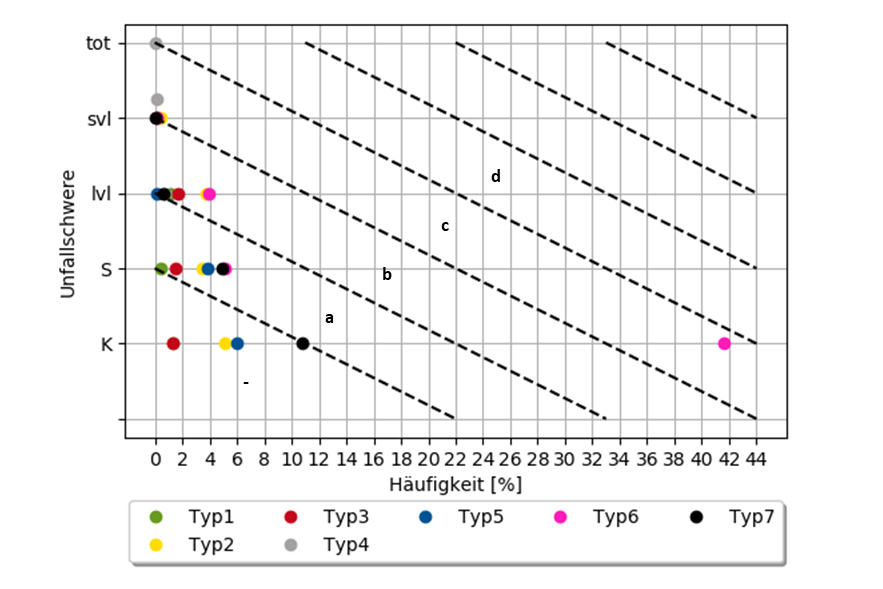
\includegraphics[width=12cm,height=8cm]{figures/Bewertung_UTF}
		\caption[Bewertung der Unfälle im Testgebiet anhand der sieben Unfalltypen mit Kleinunfällen]{Bewertung der Unfälle im Testgebiet anhand der sieben Unfalltypen mit Kleinunfällen}\label{fig:Bewertung_UTF}
	\end{figure}
\end{savenotes}

In die Kategorie \textit{c} fallen die Typen 1, 2, 3, 6 und 7 da hier jeweils Unfälle mit schweren Verletzungen auftraten. Abbildung \ref{fig:Bewertung_UTF(2)} im Anhang \ref{chapter:Bewertungsdiagramme} stellt vergrößerte Ausschnitte der Abbildung \ref{fig:Bewertung_UTF} zu besseren Verständlichkeit dar. Die Unfälle mit dem Typ 6 werden nicht nur aufgrund der Verletzungen mit der Kategorie \textit{c} bewertet, sondern auch aufgrund der hohen Anzahl, ca. 41,5 \%, an Kleinunfällen bei denen der Typ 6 angegeben wurde. Der Unfalltyp 5 wird, wie zuvor, mit der Kategorie \textit{b} bewertet.

Anhand der sieben Unfalltypen ist zwar eine Bewertung der Unfälle möglich, die Aussagekraft ist jedoch relativ gering, da der Unfalltyp wenig Informationen über den Unfallhergang preis gibt. Zur genaueren Beschreibung wurden die Feintypen nach GDV verwendet. Im Folgenden werden die sieben Unfalltypen anhand der aufgetretenen Feintypen analysiert. Aufgrund der hohen Anzahl der Feintypen werden nur die Unfälle denen die Risiko-Kategorie \textit{d}, \textit{c} oder \textit{b} zugeordnet wurde genauer beschrieben. Die restlichen Feintypen können aus den jeweiligen Diagrammen entnommen werden.

\subsubsection{Feintypen Unfalltyp 1}


\begin{savenotes}
	\begin{figure}[H]
		\centering
		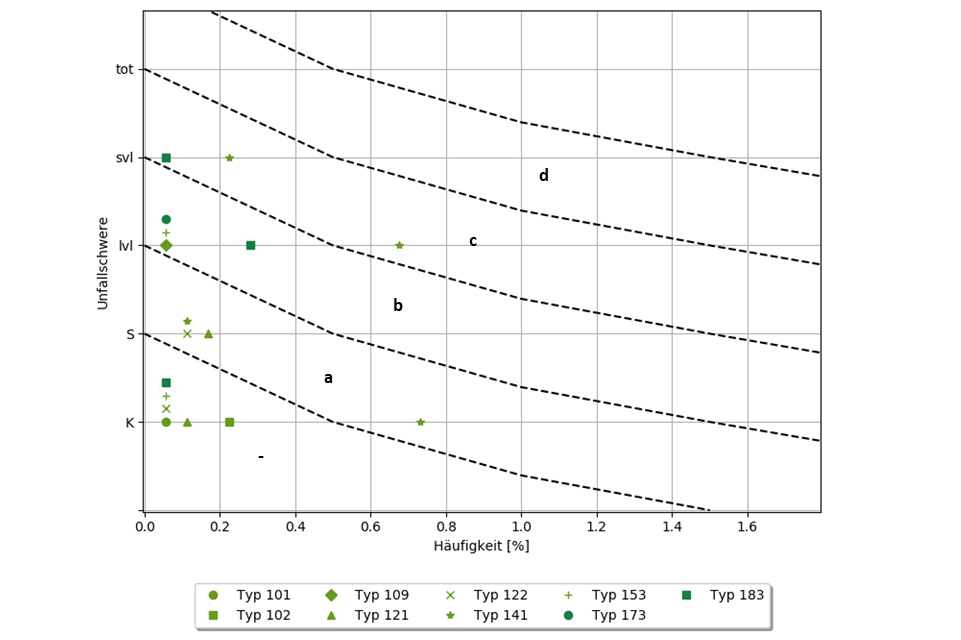
\includegraphics[width=12cm,height=8cm]{figures/Bewertung_FT1}
		\caption[Bewertung der Unfälle, denen ein Feintyp des Unfalltyps 1 zugeordnet wurde]{Bewertung der Unfälle, denen ein Feintyp des Unfalltyps 1 zugeordnet wurde}\label{fig:Bewertung_FT1}
	\end{figure}
\end{savenotes}

\subsubsection{Feintypen Unfalltyp 2}


\begin{savenotes}
	\begin{figure}[H]
		\centering
		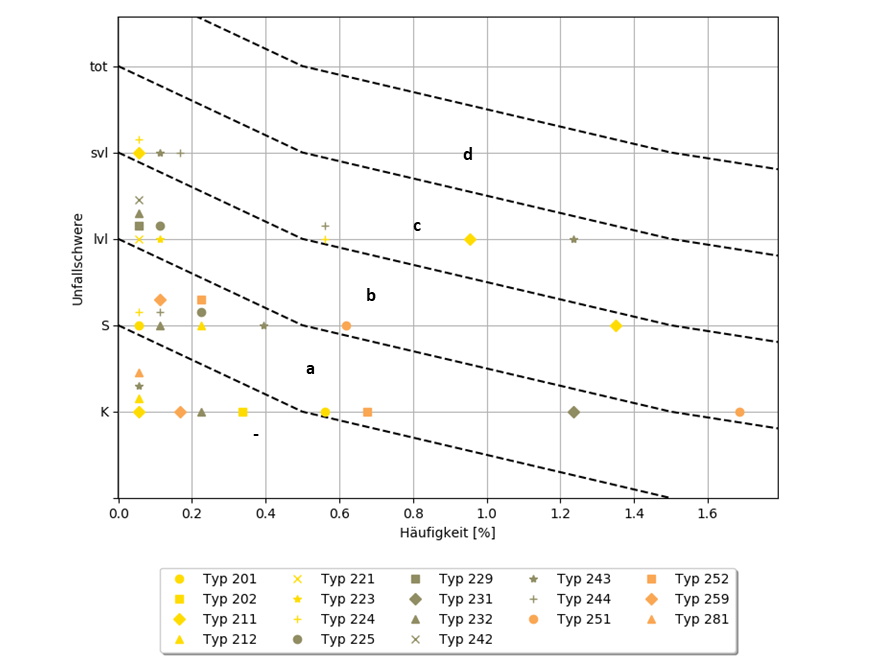
\includegraphics[width=12cm,height=8cm]{figures/Bewertung_FT2}
		\caption[Bewertung der Unfälle, denen ein Feintyp des Unfalltyps 2 zugeordnet wurde]{Bewertung der Unfälle, denen ein Feintyp des Unfalltyps 2 zugeordnet wurde}\label{fig:Bewertung_FT2}
	\end{figure}
\end{savenotes}

\subsubsection{Feintypen Unfalltyp 3}


\begin{savenotes}
	\begin{figure}[H]
		\centering
		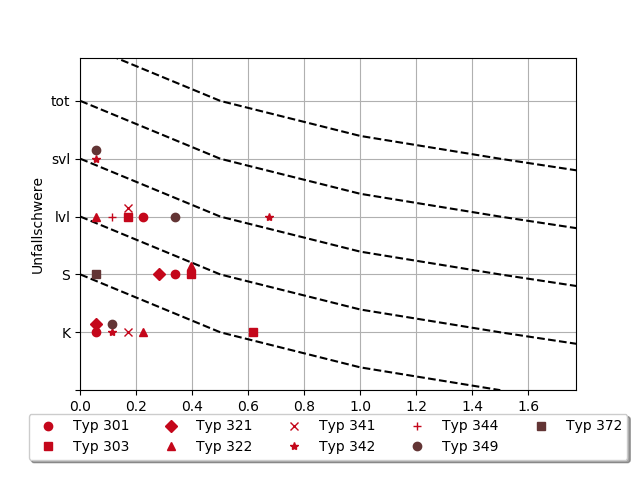
\includegraphics[width=12cm,height=8cm]{figures/Bewertung_FT3}
		\caption[Bewertung der Unfälle, denen ein Feintyp des Unfalltyps 3 zugeordnet wurde]{Bewertung der Unfälle, denen ein Feintyp des Unfalltyps 3 zugeordnet wurde}\label{fig:Bewertung_FT3}
	\end{figure}
\end{savenotes}

\subsubsection{Feintypen Unfalltyp 4}


\begin{savenotes}
	\begin{figure}[H]
		\centering
		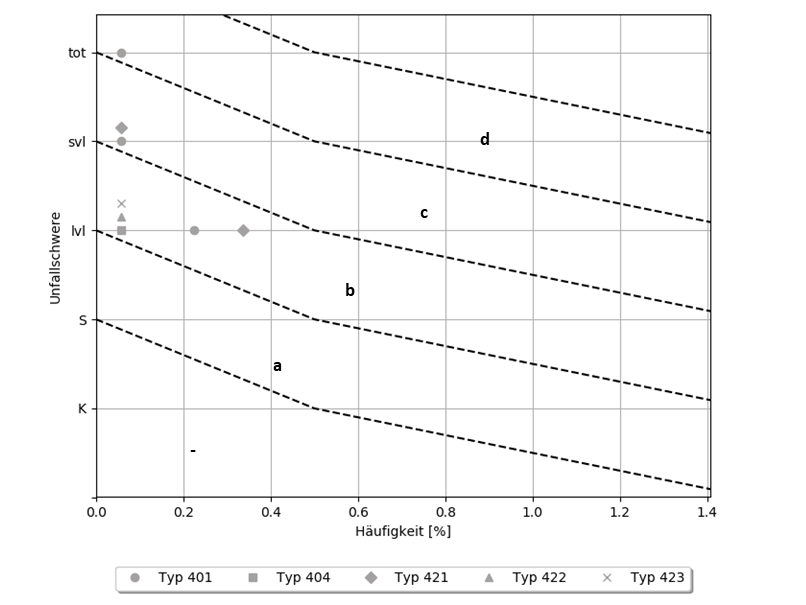
\includegraphics[width=12cm,height=8cm]{figures/Bewertung_FT4}
		\caption[Bewertung der Unfälle, denen ein Feintyp des Unfalltyps 4 zugeordnet wurde]{Bewertung der Unfälle, denen ein Feintyp des Unfalltyps 4 zugeordnet wurde}\label{fig:Bewertung_FT4}
	\end{figure}
\end{savenotes}

\subsubsection{Feintypen Unfalltyp 5}


\begin{savenotes}
	\begin{figure}[H]
		\centering
		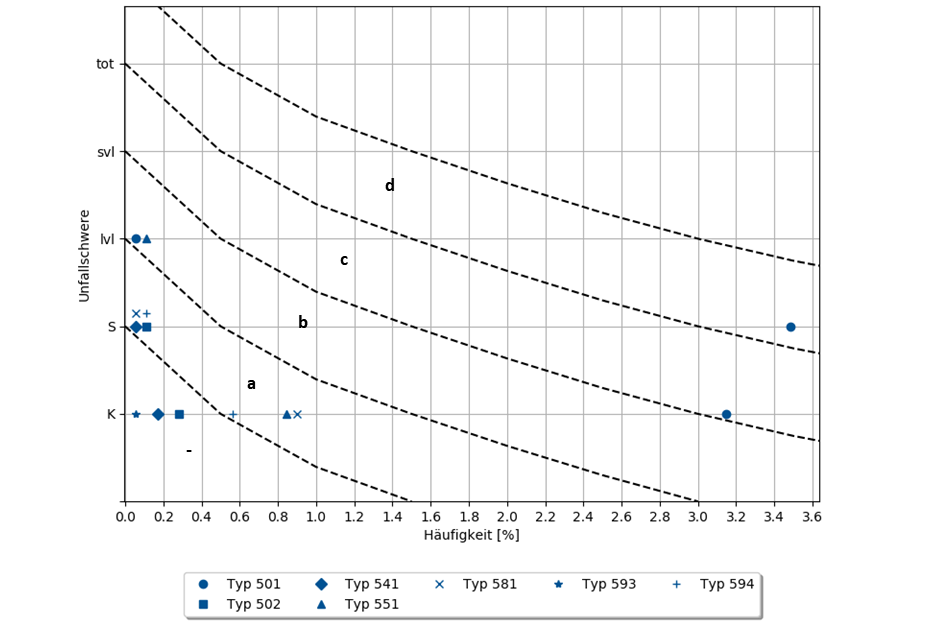
\includegraphics[width=12cm,height=8cm]{figures/Bewertung_FT5}
		\caption[Bewertung der Unfälle, denen ein Feintyp des Unfalltyps 5 zugeordnet wurde]{Bewertung der Unfälle, denen ein Feintyp des Unfalltyps 5 zugeordnet wurde}\label{fig:Bewertung_FT5}
	\end{figure}
\end{savenotes}

\subsubsection{Feintypen Unfalltyp 6}


\begin{savenotes}
	\begin{figure}[H]
		\centering
		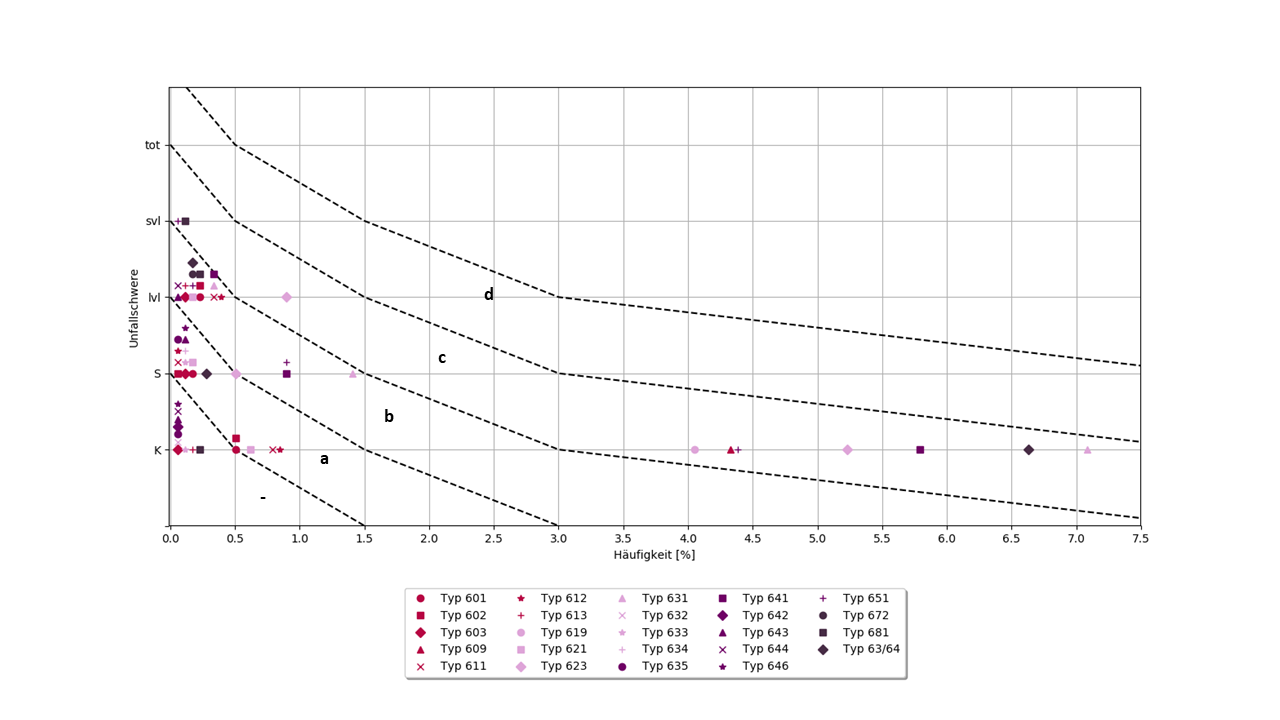
\includegraphics[width=18cm,height=10cm]{figures/Bewertung_FT6}
		\caption[Bewertung der Unfälle, denen ein Feintyp des Unfalltyps 6 zugeordnet wurde]{Bewertung der Unfälle, denen ein Feintyp des Unfalltyps 6 zugeordnet wurde}\label{fig:Bewertung_FT6}
	\end{figure}
\end{savenotes}

\subsubsection{Feintypen Unfalltyp 7}


\begin{savenotes}
	\begin{figure}[H]
		\centering
		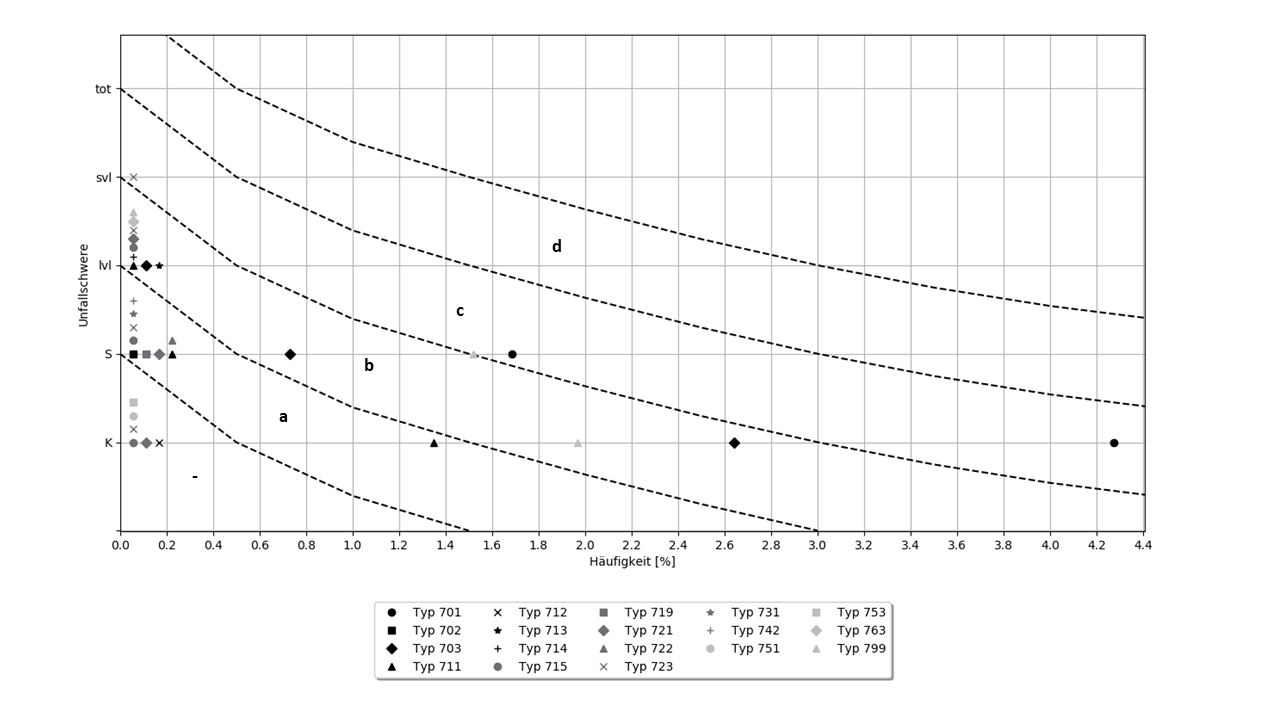
\includegraphics[width=18cm,height=10cm]{figures/Bewertung_FT7}
		\caption[Bewertung der Unfälle, denen ein Feintyp des Unfalltyps 7 zugeordnet wurde]{Bewertung der Unfälle, denen ein Feintyp des Unfalltyps 7 zugeordnet wurde}\label{fig:Bewertung_FT7}
	\end{figure}
\end{savenotes}

\section{Zuordnung der Unfälle zu Fahrsituationen}\label{section:Zuordnung der Unfälle zu Fahrsituationen}
%Mit hilfe der Excel in der den Fahrssituationen mögliche Unfalltypen und Ursachen zugeordnet wurden.

%Erke stellt im Anhang (Anhang 5) verschiedene Konflikttypen mit den dazugehörigen amtlichen Unfallursachen dar. Diese werden im Text ab S.23 erläutert. Gleiche Ursachen können der Auslöser für verschiedene Konflikte sein. Könnte bei der Typisierung der Kleinunfälle hilfreich sein.

%Fastenmeier hat ein Klassifikationsmuster für Verkehrssituationen aufgestellt in \parencite[S.67]{Gerstenberger.17.02.2015}.

%Gerstenberger hat Knotenpunktunfallgruppen erstellt, diese können vllt. bei den Unfällen an Knotenpunkten im Testgebiet angewendet werden. Vgl. S.90 und Anhang 5. Die Knotenpunktunfallgruppen fassen die Unfalltypen nach GDV zusammen.

%Crash Cost Estimates by Crash Type, kann evtl. verwendet werden um kritische urbane Fahrsituationen zu nennen (Advanced Road Safety Concepts 8. p.91)

%Bewertung auch gleich hier mit rein.

\section{Unfallhäufungsstellen/Unfallschwerpunkte}
%Um markante Punkte der Teststrecke ausfindig zu machen werden zunächst alle Unfälle auf einer Übersichtskarte dargestellt und dann Auffälligkeiten genauer betrachtet.

%Adrian S.7 Unfalldichte wird ermittelt und in einer Hatmap dargestellt. Auffällige Punkte nennen.
%Heatmap/Übersichtkarte
%Unfälle an den UHS genauer anschauen, vllt. kann  man mit den Kurzbeschreibungen die Feintypen bestimmen.

%Unfallauffällige Knotenpunkte nach den Anforderungen der FGSV überprüfen. Gibt es Anforderungen die nicht eingehalten werden? Gerstenberger gibt auf den Seiten 10 bis 14 einen Überblick über die Anforderungen. Evtl Sichtbereich und Fußgänger/Radfahrerführung + Abbiegeströme anschauen.

%\parencite[S.114]{Gerstenberger.17.02.2015} nennt wichtige Faktoren, die bei der Bewertung von Unfallhäufungen berücksichtigt werden sollten. Hier ist die Verkehrsstärke in der bevorrechtigten und der wartepflichtigen Zufahrt, sowie die Art der Lichtsignalsteuerung zu berücksichtigen. Zudem stellt er in seiner Arbeit fest, dass zur entsprechenden Bewertung des Unfallgeschehens immer die aktuellen lokalen Begebenheiten mit in die Betrachtung einbezogen werden müssen.

%Bei der Auswertung der Unfälle an Knotenpunkten, zählen alle Unfälle zum Knotenpunkt, die sich bis zu 25 m in den Knotenpunktarm hinein ereignen. (FGSV)

%Gründl erwähnt potenzielle Gefahrenquellen auf S.102. Trifft hier was zu?

\section{Zwischenfazit}

%Um Unfälle rekonstruieren zu können werden weit aus mehr Daten, als in dieser Arbeit zur Verfügung stehen, benötigt. Hier liegen nur Allgemeine Unfalldaten wie z.B. die Unfalltyp, Unfallart, Charakteristik und Besonderheit der Unfallstelle und Angaben zu den  Beteiligten vor. Diese Daten reichen für eine Klärung der Schuldfragen. Für die Unfallforschung sind darüber hinaus Daten des Unfallorts und des Unfallfahrzeugs in denen z.B. die Reifenspuren oder Spuren am Fahrzeug angegeben werden genauso von Bedeutung. Sie werden benötigt, um  genau ermitteln zu können, wie es zu einem Unfall kam \parencite[S.28]{Burg.2017}.

%Erster Teil wurde mit dem Datensatz ohne Kurzsachverhalte bearbeitet, da diese erst später zu Verfügung standen. Evtl. würden Unfälle dazu kommen. Da mit den Kurzsachverhalten mehr Informationen zu den Kleiunfällen gegeben sind. Könnte also nochmals überarbeitet werden.

%\section{Sonstiges}

%Reichart gibt an, dass für den Vergleich von Betrachtungseinheiten die Fehler- bzw. Unfallrate von bedeutung ist. Näheres findet sich in seiner Arbeit an S.20.

%"Wenn Fahrer nicht von sich aus Fehler zugeben, dann sind sie der Polizei nicht bekannt und stehen auch nicht in der Verkehrsunfallanzeige." \parencite[S.27]{Grundl.2005}

%\enquote{Bestimmte Merkmale der Straßeninfrastruktur wirken sich nur auf Teilkollektive der Verkehrsteilnehmer aus oder besitzen je nach Unfallkonstellation auch unterschiedliche Wirkungen} \parencite[S.85]{Aurich.2015}.

%\subsection{Unfallursachen}

%Es gibt häufig nicht nur eine Unfallursache, sondern verschiedene Rahmenbedingungen mit negativem Einfluss auf die Verkehrssituation. (FGSV)

%Unfälle haben im Schnitt 1,4 Ursachen. Die Hauptunfallursachen beim Fahrzeugführer sind Fehler beim Abbiegen, Wenden, Rückwärtsfahren sowie beim Ein- und Anfahren. Am Zweithäufigsten wird die Vorfahrt bzw. der Vorrang anderer missachtet. \parencite[S.149]{StatistischesBundesamt.2016}